% !TeX program = pdfLaTeX
\documentclass[smallextended]{svjour3}       % onecolumn (second format)
%\documentclass[twocolumn]{svjour3}          % twocolumn
%
\smartqed  % flush right qed marks, e.g. at end of proof
%
\usepackage{amsmath}
\usepackage{graphicx}
\usepackage[utf8]{inputenc}

\usepackage[hyphens]{url} % not crucial - just used below for the URL
\usepackage{hyperref}
\providecommand{\tightlist}{%
  \setlength{\itemsep}{0pt}\setlength{\parskip}{0pt}}

%
% \usepackage{mathptmx}      % use Times fonts if available on your TeX system
%
% insert here the call for the packages your document requires
%\usepackage{latexsym}
% etc.
%
% please place your own definitions here and don't use \def but
% \newcommand{}{}
%
% Insert the name of "your journal" with
% \journalname{myjournal}
%

%% load any required packages here




\usepackage{booktabs}
\usepackage{longtable}
\usepackage{array}
\usepackage{multirow}
\usepackage{wrapfig}
\usepackage{float}
\usepackage{colortbl}
\usepackage{pdflscape}
\usepackage{tabu}
\usepackage{threeparttable}
\usepackage{threeparttablex}
\usepackage[normalem]{ulem}
\usepackage{makecell}
\usepackage{xcolor}

\begin{document}

\title{Do moral communities have a spatial dimension? A spatial exploratory
analysis of places of worship and violent crime in the city of Recife,
Brazil \thanks{Grants or other notes about the article that should go on the front page
should be placed here. General acknowledgments should be placed at the
end of the article.} }


    \titlerunning{Moral communities and crime}

\author{  Author One \and  Author Two \and  Author Three \and  Author Four \and  }


\institute{
        Author One \at
     A Department, University of XXX \\
     \email{\href{mailto:abc@example.edu}{\nolinkurl{abc@example.edu}}}  %  \\
%             \emph{Present address:} of F. Author  %  if needed
    \and
        Author Two \at
     A Department, University of XXX \\
     \email{\href{mailto:def@example.edu}{\nolinkurl{def@example.edu}}}  %  \\
%             \emph{Present address:} of F. Author  %  if needed
    \and
        Author Three \at
     A Department, University of XXX \\
     \email{\href{mailto:ghi@example.edu}{\nolinkurl{ghi@example.edu}}}  %  \\
%             \emph{Present address:} of F. Author  %  if needed
    \and
        Author Four \at
     Some School, University of WWW \\
     \email{\href{mailto:jkl@school.edu}{\nolinkurl{jkl@school.edu}}}  %  \\
%             \emph{Present address:} of F. Author  %  if needed
    \and
    }

\date{Received: date / Accepted: date}
% The correct dates will be entered by the editor


\maketitle

\begin{abstract}
Religious tenets of the type ``thou shalt not kill'' and their
equivalents in many world religions have functioned as \emph{de facto}
social policy for determining appropriate and acceptable behavior over
the centuries. With the advent of the scientific study of religion,
there has been a growth of interest in the role of religions to operate
as moral communities. Moral communities, a concept closely related to
informal social control, are of interest in countries and regions where
formal controls are weak and ineffective. The objective of this paper is
to present a spatial analysis of Violent and Intentional Crime in the
city of Recife in Brazil, with a focus on the possible interactions
between criminal events and places of worship. Previous research into
moral communities has advocated the need for analysis at different
scales, and this analysis contributes to the literature by using
micro-level data and appropriate spatial analytical tools for spatial
point patterns. Analysis is conducted using three different types of
places of worship (Catholic, Evangelical, and Spiritist) and three types
of business establishments as controls (ice cream shops, pharmacies, and
supermarkets). The results suggest that Catholic places of worship do
not project moral communities geographically more than, say, ice cream
shops. The intensity of criminal events in the proximity of Evangelical
places of worship, in contrast, is markedly higher at short distances
than for any of our other referential events; however, at distances
between 300 and 500 m the intensity is lower. Finally, the intensity of
crime with respect to Spiritist churches, albeit lower at short
distances, tends to be significantly higher at distances between 300 and
500 m.
\\
\keywords{
        Moral communities \and
        Crime \and
        Places of worship \and
        Point pattern analysis \and
        Intensity \and
    }


\end{abstract}


\def\spacingset#1{\renewcommand{\baselinestretch}%
{#1}\small\normalsize} \spacingset{1}


\hypertarget{intro}{%
\section{Introduction}\label{intro}}

Violent crime is a widespread phenomenon with negative impacts on many
spheres of life and society. Although the rate of homicides worldwide
has grown at a slower rate than the population in the past few decades,
the number of people killed in homicides still increased from 362,000 in
1990 to 464,000 in 2017 (United Nations Office on Drugs and Crime
2019a). Furthermore, variations in the prevalence of violent crime tend
to be extremely uneven. The Americas, with a population of approximately
793.8 million people in 2019 (or about 10.3\% of the world population),
accounted for approximately 173,000 homicides in 2017, or approximately
37.3\% of all homicides in the world. Within the Americas, Brazil (along
with Venezuela, Colombia, and Mexico) is one of the largest countries in
the region with high homicide rates. And there are notable variations at
the sub-national and intra-metropolitan levels as well. In fact,
understanding the variations in the prevalence of violent crime is
recognized as key to achieving policy goals:

\begin{quote}
\begin{quote}
High levels of homicidal violence are concentrated in geographic and
demographic ``pockets'', so achieving target 16.1 of the Sustainable
Development Goals requires interventions within the specific regions,
countries, communities and population groups that are most at risk
(United Nations Office on Drugs and Crime 2019a, 35)
\end{quote}
\end{quote}

This concern is not idle: violent crime tends to be more acute in those
regions most in need of development. On the one hand, violent crime
represents an economic and social drag (Becker and Kassouf 2017). The
impacts are multifaceted, since they affect people's well-being, either
through the loss of human life, mental health, and limitations in the
right to public spaces (Doran and Burgess 2011), or through disturbances
in schooling and academic achievement (United Nations Office on Drugs
and Crime 2019b). In turn, these negative effects combine to create the
unfortunate conditions that tend to breed criminal behavior, thus
creating a vicious cycle of economic disadvantage and violence (United
Nations Office on Drugs and Crime 2019b). It is not surprising, given
these peculiarities, that researchers have joined calls for increased
attention to the study of the patterns of violent crime in Low and
Middle Income Countries (LMIC; Murray, Cerqueira, and Kahn 2013).

Added to the scenario, formal social control institutions in countries
like Brazil often leave something (or much) to be desired: while in
practice they should inhibit criminal behavior, they suffer from deep
deficiencies that end up eroding the deterrent power of the justice
system. Serious institutional problems include the inefficiency of the
police, the lack of national legislation, the glacial pace of judicial
processes, and the weak situation of the prison system in the country
(Menezes et al. 2013). This makes it even more urgent to understand the
role of \emph{informal social controls}, i.e., the ability of community
organizations such as schools, clubs, and neighborhood associations to
suppress crime by strengthening the capabilities of neighbors to control
inappropriate behavior (Groff 2015).

In order to understand the factors that can potentially help to deter
crime, beyond formal control, it is important to identify empirical
regularities. Criminological factors include concrete elements (such as
the presence of arms or drugs, or elements of the built environment),
and also figurative factors, which include the social cost of deviant
behavior. Accordingly, a number of studies have investigated various
aspects of the environment and neighborhood design (e.g., Foster,
Giles-Corti, and Knuiman 2010; He, Páez, and Liu 2017; Loukaitou-Sideris
et al. 2001), whereas other studies have focused on exposure to
environmental attributes that signal weakened norms, such as liquor and
tobacco outlets (e.g., Brower and Carroll 2007; Deryol et al. 2016;
Lipton et al. 2008; Quick, Law, and Luan 2017).

Yet another fruitful avenue for research, and one that has only recently
begun to be explored, is the presence of environmental attributes that
can help to reinforce moral norms, such as schools and churches (e.g.,
Abdullah et al. 2018; Davignon and Thomson 2015; Furr-Holden et al.
2010; Traunmuller 2011). It is thus that in a recent paper, Warner and
Konkel (2019) note that the role of places of worship, as distinct
entities from the members of the congregations, have received less
attention in empirical and theoretical research for their deterrence
potential. The role of these institutions might be particularly
important in places where formal state institutions lack the means or
the will to enforce norms in a consistent way - as is the case in Brazil
(Garmany 2014).

With the above considerations in mind, the objective of this paper is to
investigate whether and how places of worship correlate spatially with
criminal events, or in other words, to investigate whether their signals
as moral communities have a discernible spatial dimension. Our argument
is as follows:

\begin{enumerate}
\def\labelenumi{\arabic{enumi}.}
\item
  Since places of worship are associated with normative codes of
  behavior, can they by their presence contribute to create moral
  communities? The mechanisms for this are explained by Groff (Groff
  2015) in terms of ``Eyes on the Street'' (see Jacobs 1961, 1968;
  Appleyard 1980) and Human Territorial Functioning (Taylor 1988, 1998).
\item
  If so, what is the distance decay of said moral community effect? Is
  it uniform over a certain distance, such that it could be well
  approximated by areas, or does it vary?
\end{enumerate}

The case study is the city of Recife in the state of Pernambuco, in
Brazil's Northeast. Recife is a large and important metropolitan area in
a historically poor region, and afflicted by high levels of violent
crime, having the dubious honor of being one of five state capitals with
the highest rates of homicide in the period under study (Menezes et al.
2013). The empirical strategy is to use spatial analysis to explore the
potential geographical relationships between violent criminal events, on
the one hand, and places of worship and a selection of commercial
establishments that serve as controls, on the other.

Note that this is a reproducible research document. The analysis is
implemented using the \texttt{R} statistical computing language, and
documents to replicate the analysis, in addition to all data necessary,
are available from a
repository\footnote{\url{https://drive.google.com/open?id=1tuJM4Mhi0Ftq3ZEwjv6RP9vO3veGjIR_}}.

\hypertarget{background}{%
\section{Background}\label{background}}

\hypertarget{theoretical-perspectives-on-religion-and-crime}{%
\subsection{Theoretical Perspectives on Religion and
Crime}\label{theoretical-perspectives-on-religion-and-crime}}

Why do humans behave morally? For millennia, it has been the role of
religion to provide the basic tenets of morally acceptable behavior:
thou shalt not kill et al., and their equivalent in many world religions
(e.g., Donovan 1986). Enforcement of such tenets implies different
mechanisms, including \emph{sin}, \emph{haram}, \emph{karma}, and
\emph{tapu}, with punishment delivered by hellfire and exile to
\emph{Jahannam} or \emph{Gehenna}, to mention just some choice places of
torment. In addition to acting as \emph{de facto} social policy for much
of history, many of these religious tenets still have the force of law
in many cultures and regions - and even where they do not, they are held
by some researchers and policy experts to be helpful complements to
reduce crime in any case (e.g., Durrant and Poppelwell 2017; Johnson
2011). The hypothesis that religion can act as a factor that deters and
reduces criminal behavior, therefore, has prompted the scientific study
of the effectiveness of religion on moral behavior (Hoffmann 2015).

An early effort to theorize the effect of religion on criminal behavior
was the \emph{hellfire hypothesis} of Hirschi and Stark (1969). The
focus of this hypothesis is the threat of extra-temporal (and possibly
eternal) punishment, and how this threat can deter believers from
commandment-breaking (also see Pascal's wager). Accordingly, Hirsch and
Stark (1969) posit that negative correlations between crime and religion
are a consequence of a sense of commitment with normative values, a
commitment that is ritually reinforced in a regular fashion (e.g., the
liturgical rite of peace in Catholic Mass). Rohrbaugh and Jessor (1975),
for instance, note that by attributing to divinity (or some other
supra-terrenal entity) the supreme force of punishment, religion helps
to build a sense of obduracy, or ``hardening'' against temptation.

Despite its intuitive appeal, research has not provided much direct
evidence for the hypothesis of hellfire (Hoffmann 2015, 1). In a bizarre
twist, even mainstream doctrines (such as absolution) may in fact
encourage beliefs that neutralize the fear of \emph{terrenal}
punishment, and thus turn out to be criminogenic (e.g., Topalli,
Brezina, and Bernhardt 2013). More deviant cases can even recast
criminal behavior as a form of spiritual insurgency (Chesnut 2017).
Counterexamples like this notwithstanding, researchers remain open to
the possibility that ``religion may still serve as a social control
mechanism by encouraging conventional beliefs, monitoring behaviors,
enhancing family attachments, or providing conventional activities''
(Hoffmann 2015, 1). In this way, the hypothesis of \emph{moral
communities} (Stark 1996) recognizes that social integration is
essential for increasing social control, thus reducing the practice of
behavior that is not in accordance with current norms. Rohrbaugh and
Jessor (1975) also emphasize that religion acts as social control since
it defines what is an appropriate attitude according to moral values,
thus making moral communities a close relative of the concept of
\emph{informal social control}, defined as ``the ability of social
groups or institutions to make norms or rules
effective''\footnote{The discussion about disorder is directly related to the idea of social control. According to this perspective, control mechanisms to contain deviant actions are considered indispensable [@Rodrigues2012medo]. This theory assumes that the deviant act is seen as normal in social organization, and coercive forces are needed to limit such impulses. This control can be exercised through formal institutions, as well as through informal mechanisms. It would be a set of norms as well as positive and negative sanctions, which are specified throughout the socialization process, which aims to establish values and build the individual's morals, disciplining society and subjecting individuals to standards and principles predefined. As the individual finds himself more and more inserted in the social context, less will be the chances of criminal behavior. From this perspective, the existence of bonds of solidarity and trust would be relevant for the effective exercise of supervision over crime in the neighborhood. Informal control is then linked to the ability of a neighborhood to establish communication and surveillance networks, interfering in cases of criminal actions and increasing security in the region.}
(Reiss 1951, 196; cited in Groff 2015, 91).

The hypothesis of moral communities has over the years been used to
examine a variety of outcomes of interest. Recent examples include
Stroope and Baker's (2018) exploration of religiosity and self-rated
health; Davignon and Thomson (2015) with their research on institutional
context and the religiosity of students; and the study of religion as a
source of trust of Traunmuller (2011). This is in addition, of course,
to numerous studies on criminal behavior such as Eitle (2011), an author
who explored the deterrence power of religion on gambling; Lee and
Bartkowski's (2004) investigation of juvenile homicide in rural areas;
and the research of Regnerus (2003) on adolescent delinquency. The
hypothesis of moral communities as a form of informal social control, on
the other hand, has been less studied from a geographical perspective,
and it is only recently that has attracted the attention of researchers.
Groff (2015), for instance, discusses informal social control as a
phenomenon that can plausibly operate at different geographical scales,
from the level of the home and family, through the street block and
neighborhood, possibly to other scales such as the county. In this way,
Nie and Yang (2019) remark on a recent paper on the lack of research
conducted to study how the religious context of a geographical area
(e.g., a county) may influence (youth smoking) behavior (p.~2). This
point is echoed by Warner and Konkel (2019), who moreover recommend the
use of smaller units of analysis (e.g., Census Block Groups), in an
effort to reduce aggregation bias (see Hipp 2007), but more importantly
because the processes defined by social disorganization
theory\footnote{The social disorganization theory (Shaw e McKay, 1942)  presents the social structure as an indispensable factor for the elaboration of theoretical and methodological models related to crime in urban neighborhoods. According to Villareal e Silva [-@Villarreal2006social], “neighborhoods characterized by dense social networks will experience greater trust among residents and cooperation in the enforcement of social norms against crime. Disadvantaged neighborhoods are thought to have fewer social ties among residents and lower rates of organizational participation”. The argument is that community characteristics such as poverty, ethnic heterogeneity and residential mobility disrupt the social organization of urban neighborhoods in such a way as to reduce their capacity to exercise social control [@Rodrigues2012medo]. Thus, aspects such as residential instability or low socioeconomic status would contribute to the weakening of the community organization, increasing crime rates. This theory highlights the importance of the geography of crime and the characteristics of disorder in its analysis.}
are thought to occur at relatively small geographical scales.

Groff (Groff 2015), in particular, explains the small-scale mechanisms
that could be in operation in terms of ``Eyes on the Street'' and Human
Territorial Functioning. ``Eyes on the Street'' (see Jacobs 1961, 1968;
Appleyard 1980) refers to involvment in small civic acts by users of
public spaces, which signal social organization to an observer.
Community engagement, moreover, is engendered at small scales, as shown
by authors that include Appleyard (1980) and more recently Grannis
(2009). Human Territorial Functioning (HTF; Taylor 1988, 1998) also
provides a valuable perspective on social informal control This concept
posits that territorial functioning is a product of the shared
perceptions of individuals in regards to places, and how these
perceptions are shaped by the physical, social, and cultural
environments. For example, Paez (2013) discusses how perceptions of
safety are the outcome of a socially interactive process, and shows how
this process leads to spatial patterning at very small-scales. The
preceding review, as well as other research (2019), makes clear the need
for research at various geographical scales. From a theoretical
perspective, the social mechanisms that underpin the hypothesis of moral
communities and informal social control can happen at various
geographical scales, some of which previous research has already
addressed: the work of Nie and Yang (2019), for one, highlights the role
of processes detectable at a relatively high level of aggregation,
whereas Warner and Konkel (2019), looking specifically at the effect of
places of worship, bring the study closer to the level of the
neighborhood.

\hypertarget{religion-in-brazil}{%
\subsection{Religion in Brazil}\label{religion-in-brazil}}

Brazil is a predominantly Christian country. The first national census
that collected information on religion was in 1872, a year when
practically the entire population (99.72\%) identified themselves as
Catholic. In the 1940 census, when the religion question was asked
again, Catholicism was still the dominant religion with 95.2\% of
Brazilians declaring themselves as Catholics. The dominance of
Catholicism in the religious life of Brazil is unsurprising given the
country's past as a former colony of a Catholic power (Portugal).
However, the religious makeup of the population started to become less
homogeneous in the second half of the twentieth century. Among other
offerings in the market place of spiritual ideas, Spiritism stands out.
The Spiritist Doctrine was founded in nineteenth-century France by Allan
Kardec as a way of understanding the world and its relations with the
``beyond'', in a curious mix of pseudo-scientific language, philosophy,
and religion (Arribas 2011a). Spiritism arrived in Brazil in the middle
of the nineteenth century, and since then it slowly spread in large and
medium-sized cities. Today, Spiritism is the third largest religious
segment in Brazil, after Catholicism and Evangelical Christianism, and
shares with these religions the Christian principle of charity through
pious assistance.

Another signal event in the developmento of religion in Brazil was the
arrival of Pentecostal Protestant churches, such as the Christian
Congregation of Brazil in 1910 and the Assembly of God in 1911.
Initially, these religious denominations did not make important inroads
in Brazilian society (as evidenced by the 1940 census). However, in the
context of rapid industrialization and major urbanization, they
contributed to the change in the religious landscape along with other
religions (Souza 2019): according to the 2010 census the configuration
of the religious scene in Brazil had changed considerably from the
previous century: 64.6\% of the population identified as Catholic and
22.2\% as Evangelical Christians. The acceleration of this demographic
change was directly related to successful proselitism by Evangelical
churches: The Assembly of God, for instance, is a church that grew
considerably to total more than 12.3 million adherents. This church is
represented extensively in many regions of the country, following a
system of loosely allied ministries. With a charismatic profile and the
lack of a centralized authority, growth of this church has occurred
mainly through subdivision into numerous small and autonomous churches.
These churches have in common the Prosperity Gospel and an emphasis on
economic entrepreneurship (e.g., Mora 2008). They also do not shy away
from partisan political action.

In general, there have been two major changes in Brazil regarding
religious issues: the slow decline of Catholicism and the rapid growth
of Evangelical Christianism. These changes are evident in the daily life
of the average Brazilian, either through the radio or through TV
programs, which give more and more space to religious doctrines. At the
same time, there has been an increase in cases of religious intolerance
in Brazil, generating violence acts against temples, objects of worship,
and people (e.g., Souza 2019; Fonseca 2018).

In what follows, we propose to adopt a disaggregated approach by
considering the intensity of criminal events with respect to places of
worship. This requires micro-level data both of crimes and places of
worship, and the use of appropriate spatial analytical tools for point
patterns, as discussed next.

\hypertarget{methods}{%
\section{Empirical Strategy}\label{methods}}

As noted above, previous research that has investigated the presence of
churches from a geographical perspective has used data aggregated at
different scales. In the case of Nie and Yang (2019), the unit of
analysis was the county, whereas Warner and Konkel (2019) used Census
Block Groups, a much smaller unit of analysis. Research in spatial
criminology, on the other hand, has studied criminal events as point
patterns since at least the work of Levine et al.~(1986) investigated
the concentration of criminal events in the proximity of bus stops.
Since then, many other works have applied tools of spatial point pattern
analysis to investigate the empirical properties of the distribution of
crime. This includes Craglia et al.~(2000) who used the Ripley's
K-function (Ripley 1976) to investigate clustering processes, and
Rogerson and Sun (2001) who applied nearest neighbor techniques to the
study of arson. More recent studies of crime as point patterns are
Nakaya and Yano (2010), Kiani et al.~(2015), and Malleson and Andresen
(2015).

Readers interested in point pattern analysis techniques are urged to
consult the still valuable Bailey and Gatrell (1995) or for an
up-to-date and in-depth coverage of the topic, the excellent text by
Baddeley et al.~(2015). In this paper we will concentrate on one
property of point processes, namely the intensity. Suppose that the
outcome of interest is the number of events per unit area
\(Y(\mathcal{A})\). This could be, for instance, the number of criminal
events observed in an arbitrary area. The intensity of a point pattern
then is as follows: \[
\lambda(s)=\lim_{\text{d}s \to 0}\frac{E[Y(\text{d}s)]}{\text{d}s}
\]

\noindent where \(\lambda(s)\) is the intensity of the process at point
\(s\), given by the expected number of events in a small area
\(\text{d}s\) around \(s\), as the area becomes arbitrarily small. If
the process is homogeneous (i.e., the intensity is a constant over
space), an apt estimator of the intensity is the global intensity,
simply the number of events divided by the area of the region under
analysis: \[
\hat{\lambda} = \frac{n}{|\mathcal{A}|}
\]

When the process is not homogeneous, other estimators are more
appropriate. In the analysis to follow we use two estimators of
intensity: conditional quadrat counts and relative distribution
estimate. These techniques are briefly discussed next.

\hypertarget{conditional-quadrat-counts}{%
\subsection{Conditional Quadrat
Counts}\label{conditional-quadrat-counts}}

Quadrat counts is a relatively simple technique to analyze spatial
variations in the intensity of a point process. It operates by
partitioning the region under study \(\mathcal{A}\) into subregions
\(\mathcal{A}_1,\cdots,\mathcal{A}_m\). These subregions are mutually
exclusive, and their union is identical to \(\mathcal{A}\). In the
simplest case, the subregions have equal area. The number of events
within each subregion (i.e., \(n_{\mathcal{A}}\)) divided by the area of
the subregion (i.e., \(|\mathcal{A}|\)) is a local estimate of the
intensity: \[
\lambda(\mathcal{A}_i)=\frac{n_{\mathcal{A}_i}}{|\mathcal{A}_i|}
\]

A test for homogeneity consists of assessing whether the intensity of
the point process at the quadrats is uniform: \[
\lambda(\mathcal{A}_1)=\cdots=\lambda(\mathcal{A}_m)
\]

Using quadrats of equal size is a convenient simplification, but in
principle the areas could be different - in which case the count of
events would be proportional to the area of the quadrat under
homogeneity. An interesting variation of this technique is conditional
quadrat counts, whereby the partition of regions
\(\mathcal{A}_1,\cdots,\mathcal{A}_m\) is done to reflect an underlying
covariate of interest, say \(Z\). By introducing a covariate as a
partitioning criterion, it becomes possible to calculate estimators of
the intensity of quadrats at different levels of the value of the
covariate. For exploratory purposes, we can plot average intensity by
quadrat, and compare to the global intensity.

\hypertarget{relative-distribution-estimate}{%
\subsection{Relative Distribution
Estimate}\label{relative-distribution-estimate}}

Conditional quadrat counts allow us to explore whether the intensity of
the process depends on a covariate \(Z\). A different way of expressing
this is as follows: \[
\lambda(s)=\rho\big(Z(s)\big)
\]

In this case, the intensity is a function \(\rho\) that maps how the
intensity depends on covariate \(Z\). Non-parametric estimation of
\(\rho\) uses the ratio of the density of covariate values at the
locations of the point process, relative to the \emph{spatial
distribution function} \(G\), the density of covariate values at random
locations (see Baddeley, Rubak, and Turner 2015, 179).

The density of covariate values at the locations of the is obtained by
means of a kernel density estimator, for example: \[
\lambda_0(s) = \frac{1}{|\mathcal{A}|}\sum_{i = 1}^n\kappa(Z(s_i) - z)
\] where \(s_i\) are the locations of the points.

On the other hand, \(G\) which is the cumulative distribution function
of \(Z\) at random point \(S\) uniformly distributed in \(\mathcal{A}\)
: \[
G(z) = \frac{1}{|\mathcal{A}|} \int_{\mathcal{A}}\text{I}\{Z(s)\leq z\}\text{d}s
\] where \(\text{I}\) is an indicator function that takes the value of
\(1\) if the argument is true, and the value of \(0\) otherwise. In
practice, the spatial distribution function is approximated based on a
discretization of space using a fine grid of pixels as follows: \[
G(z) = \frac{\#\{\text{pixels }s:Z(s)\leq z\}}{\# \text{pixels}}
\]

Therefore, an estimator of \(\rho\) is as follows: \[
\rho(z) = \frac{1}{|\mathcal{A}|G'(z)}\sum_{i=1}^n\kappa(Z(s_i) - z)
\] where the derivative \(G'\) can be approximated by differentiating a
smoothed estimated of \(G\). Other estimators are discussed by Baddeley
et al.~(Baddeley, Rubak, and Turner 2015, 180).

It is possible to adjust the relative distribution estimate by means of
a baseline; a baseline in this case can be a function of other
covariates that might confound the estimates of the relative
distribution, so that the relative intensity \(\lambda(s)/B(s)\) can be
assumed to depend only on covariate \(Z\). Therefore: \[
\lambda(s) = \rho(Z(s))B(s)
\] where \(B(s)\) is a baseline function. It can be seen that
\(\rho(z)=1\) is the baseline intensity; values of \(\rho(z)>1\)
correspond to intensities higher than the baseline \emph{as a function
of} \(Z(u)\), whereas values of \(\rho(z)<1\) correspond to intensities
lower than the baseline, again as a function of \(Z(u)\).

\hypertarget{interpretation}{%
\subsection{Interpretation}\label{interpretation}}

Both quadrats and the relative distribution function are estimators of
intensity. In the case of quadrats, the estimator is the number of
events in the quadrat divided by area of the quadrat (conditional
quadrat counts use irregular quadrats that are defined based on some
control variable, in our case SED). In the case of the relative
distribution, the output is an estimate of intensity conditioned on
distance from a signal event, e.g., a place of worship. The relative
distribution can be adjusted by means of a baseline function \(B(s)\),
which is also an estimate of intensity but conditioned on some control
covariate (in our cases SED). Therefore, the interpretation of the
relative distribution with a baseline function is as a ratio of the
intensity with respect to distance, to the baseline intensity according
to the control covariate. If the ratio, which is dimensionless, is 1,
then intensity as a function of distance is equal to the baseline
intensity.

\hypertarget{case}{%
\section{Case Study: Context and Data}\label{case}}

The study is of the city of Recife, the capital of the state of
Pernambuco in the Northeast region of Brazil. With a population of
1,550,390 million inhabitants in 2010, Recife is one of the main
Brazilian metropolises, exerting a great economic influence in
neighboring regions. However, the city experiences a serious problem
with violent crime, and has the dubious honor of being one of the five
capital cities in Brazil with the highest homicide rates in the period
under
study\footnote{The appendix included information that allows a more in-depth characterization of the city of Recife: population distribution, income, inequality, urban facilities (education and health) and location of residential areas.}
(Menezes et al. 2013).

In the current context, the term ``violent crime'' is an umbrella for
several forms of infractions to the penal code. Following
recommendations of the National Secretariat of Public Security of the
Ministry of Justice of 2006, these are Violent Lethal and Intentional
Crimes (VLIC; which includes intentional homicide), theft followed by
death (robbery), and corporal injury followed by death. The data on LIVC
were extracted from the Police Information System of the Secretariat of
Social Defense of Pernambuco (INFOPOL / SDS-PE), which is the most
reliable, detailed, and comprehensive information on violent deaths in
the region.

\begin{table}

\caption{\label{tab:table-descriptive-statistics}\label{tab:descriptive-statistics}Characteristics of Violent Crime in Recife, July, 2008 - June, 2009}
\centering
\begin{tabular}[t]{lr}
\toprule
 & Percentage\\
\midrule
\addlinespace[0.3em]
\multicolumn{2}{l}{\textbf{Gender of Victim}}\\
\hspace{1em}Man & 91.35\\
\hspace{1em}Woman & 8.65\\
\addlinespace[0.3em]
\multicolumn{2}{l}{\textbf{Type of Crime}}\\
\hspace{1em}Murder & 97.82\\
\hspace{1em}Robbery & 2.00\\
\hspace{1em}Body injury followed by death & 0.18\\
\addlinespace[0.3em]
\multicolumn{2}{l}{\textbf{Ethnicity of Victim}}\\
\hspace{1em}Black and Brown & 95.11\\
\hspace{1em}Yellow and White & 1.27\\
\hspace{1em}Not Reported & 3.62\\
\addlinespace[0.3em]
\multicolumn{2}{l}{\textbf{Age of Victim}}\\
\hspace{1em}1 to 12 years & 0.18\\
\hspace{1em}13 to 17 years & 11.31\\
\hspace{1em}18 to 30 years & 61.70\\
\hspace{1em}31 to 65 years & 25.84\\
\hspace{1em}65 years and older & 0.73\\
\hspace{1em}Not Reported & 0.24\\
\addlinespace[0.3em]
\multicolumn{2}{l}{\textbf{Weapon Used}}\\
\hspace{1em}Firearm & 87.51\\
\hspace{1em}Other & 12.49\\
\bottomrule
\end{tabular}
\end{table}

The data are organized at the individual level and it is possible to
obtain information about the crime event location, day of the week, day
of the month, period of the day, as well as gender, age, and race of the
victim. The database used in this study comprises the period from July
1, 2008 to June 30, 2010. Some descriptive statistics regarding this
dataset are reported in Table 1, where it can be seen that overall,
about 91\% of the victims of LIVC in the period analyzed were men, while
approximately 98\% of violent crimes were homicides. In addition, most
of the victims were black or brown, and the youth population between the
ages of 18 and 30 is the most affected by violent crime. Lastly, it
should be noted that about 88\% of the criminal events under analysis
involved firearms. Figure \ref{fig:plot-crime} shows the spatial
distribution of the 1,657 LIVC crimes that occurred in the city of
Recife between July, 2008 and June, 2010.

\begin{figure}

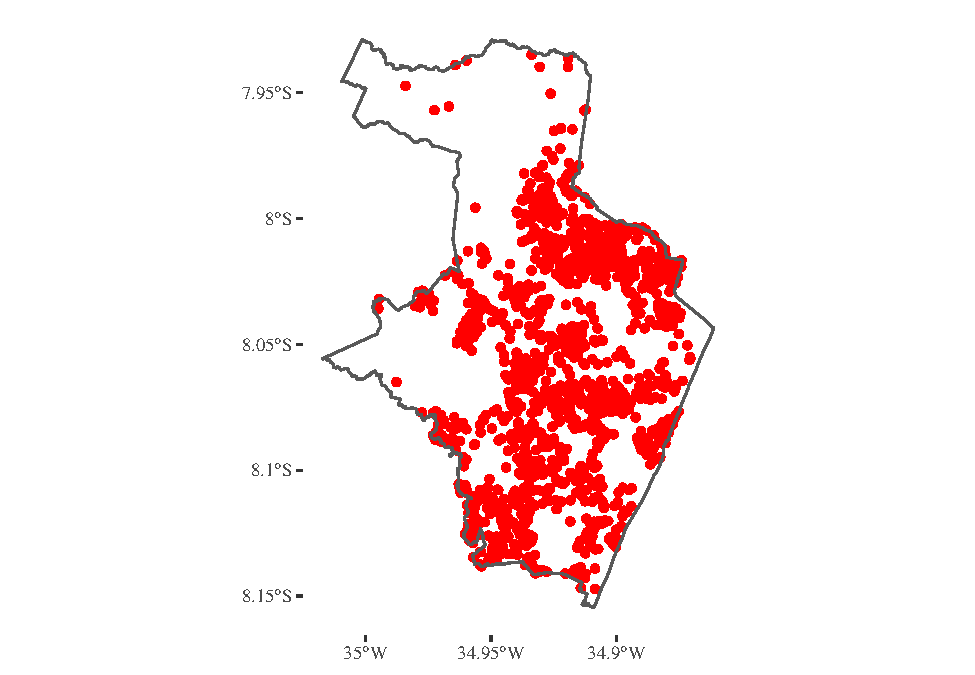
\includegraphics{Moral_Communities_and_Crime_files/figure-latex/fig-plot-crime-1} \hfill{}

\caption{\label{fig:plot-crime}Location of Lethal and Intentional Violent Crime in Recife, July, 2008 - June, 2009}\label{fig:fig-plot-crime}
\end{figure}

Information about places of interest was obtained from the National
Register of Addresses for Statistical Purposes (CNEFE - Census 2010),
which lists 78,056,411 urban and rural addresses, distributed among the
316,574 census tracts. This is the first database of its kind produced
by IBGE, and the first version was produced at the time of the 2000
Census. The way addresses are described in the National Register is very
rich, and it is possible to identify the names of the places of worship
including their denomination. Georeferencing was used to geolocate each
place of worship. In this way, a total of 1,719 places of worship were
geolocated in the city of Recife.

In addition to places of worship, the National Register of Addresses for
Statistical Purposes was queried to extract facilities other than places
of worship. To study the spatial relationship between churches and
crime, a control group was built and then a comparison of the empirical
distribution was carried out. Gilberston and Hayes (2012) highlight that
different configurations of urban space affect how people perceive the
environment around them. In this perspective, churches are continually
affecting the impression that people have of a region. Thus, we assume
that churches have unique characteristics that may or may not inhibit
the occurrence of a criminal act: they are urban constructions that are
not neutral in relation to crime. On the other hand, there are urban
facilities that do not provide any specific reason to justify the fact
that the crime occurs closer or further from these buildings. Thus, it
can be thought that any urban construction belongs to one of the
following distinct situations: neutral or non-neutral to crime.
Pharmacies, ice cream parlors and bakeries will be used in the
construction of the control group and will be considered neutral. The
comparison between the distributions of non-neutral and crime-neutral
establishments forms the empirical basis of the study. The choice of
establishments that make up the control was based on two criteria: (a)
being neutral to crime and (b) having a spatial distribution similar to
non-neutral establishments. The strategy used is to compare similar
establishments about their spatial distribution, but different in
relation to their neutrality profile in relation to crime, seeking to
simulate the existence of a case and a control group. The case will be
composed of churches, while the control will be pharmacies, ice cream
parlors and bakeries.

As discussed above, the idea is to identify points of reference that can
be used as controls, having a neutral morality profile. For the sake of
the present study, we selected pharmacies, ice cream shops, and bakeries
to construct our control group. These three types of establishments
comply with the criteria of being morally neutral and having a spatial
distribution commensurate with places of worship.

Figure \ref{fig:plot-events} shows the spatial distribution of the
places of worhsip and control establishments in the city of Recife. Note
the similarity between the maps. As expected, there are differences in
the number of points, but the locations of cases and controls are quite
similar: the distribution of the churches, as well as of the commercial
establishments follow the same pattern, being correlated with the
spatial distribution of the population (see in the appendix). Since such
urban constructions respond to society's demand, they tend to be located
close to population agglomerations.

\begin{figure}

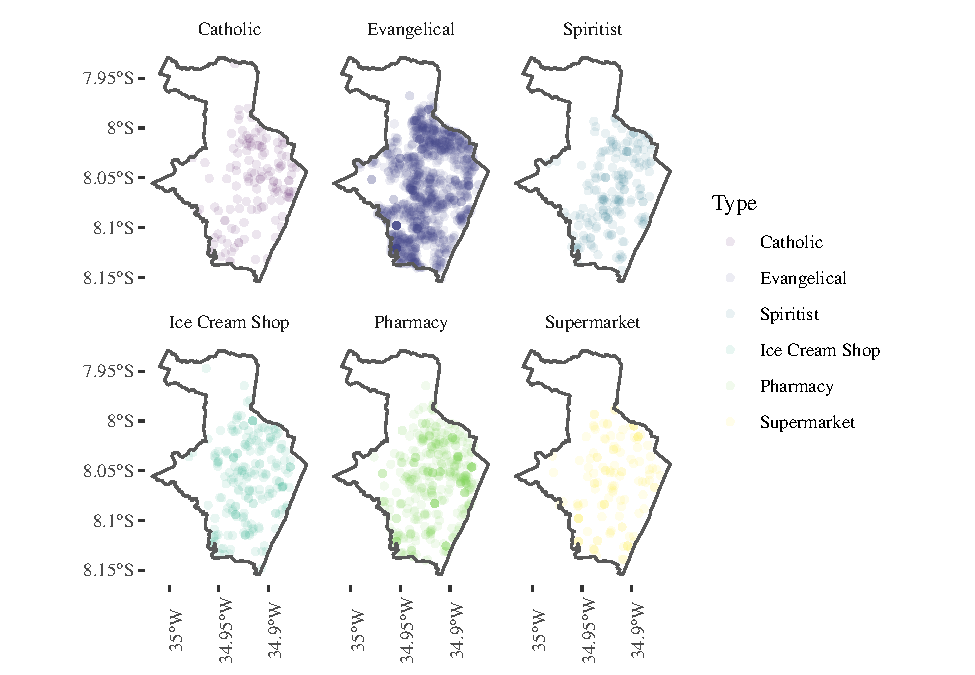
\includegraphics{Moral_Communities_and_Crime_files/figure-latex/fig-plot-events-1} \hfill{}

\caption{\label{fig:plot-events}Location of Places of Worship and Commercial Establishments in Recife}\label{fig:fig-plot-events}
\end{figure}

\hypertarget{results}{%
\section{Analysis and results}\label{results}}

\hypertarget{socio-economic-deprivation}{%
\subsection{Socio-Economic
Deprivation}\label{socio-economic-deprivation}}

The first step in our analysis is to obtain an indicator of
Socio-Economic Deprivation (SED). Socio-economic deprivation is known to
correlated positively with crime, as it often reflects relevant
criminogenic factors such as poverty and family disruption (He et al.
2015). In the present case, we have for the city of Recife information
about the variables shown in Table \ref{tab:sed-descriptive-statistics}
at the level of \emph{setores}, a small Brazilian census geography.

\begin{table}

\caption{\label{tab:table-sed-descriptive-statistics}\label{tab:sed-descriptive-statistics}Descriptive statistics of some key socio-economic and demographic variables in Recife}
\centering
\begin{tabular}[t]{lccccccc}
\toprule
Variable & Min & 2nd Quartile & Median & Mean & 3rd Quartile & Max & \makecell[l]{PC Factor 1\\ Loadings}\\
\midrule
Median Income & 122.05 & 337.40 & 581.67 & 1031.09 & 1283.79 & 181642.5 & -0.42\\
Proportion Unemployed & 0.00 & 0.05 & 0.10 & 0.10 & 0.14 & 181642.5 & 0.56\\
Proportion Poverty & 0.00 & 0.05 & 0.11 & 0.12 & 0.17 & 181642.5 & 0.58\\
Proportion Single Mother & 0.00 & 0.33 & 0.37 & 0.37 & 0.41 & 181642.5 & 0.17\\
Proportion Young Single Mother & 0.00 & 0.01 & 0.02 & 0.02 & 0.02 & 181642.5 & 0.38\\
\addlinespace
Population Density & 0.00 & 10564.16 & 16333.62 & 19230.23 & 25106.07 & 181642.5 & 0.03\\
\bottomrule
\multicolumn{8}{l}{\textit{Note: }}\\
\multicolumn{8}{l}{The variable for young single mothers is for women aged 15-25}\\
\multicolumn{8}{l}{The first principal component accounts for 44.9\% of the variance}\\
\end{tabular}
\end{table}

As seen in the table, Recife is a city with large socio-economic and
demographic disparities; for example, the \emph{setor} with the highest
median income has a median income that is 148,826\% higher than the
median income in the \emph{setor} with the lowest median income. Whereas
there are \emph{setores} where the proportion of population who are
unemployed is zero, there are \emph{setores} where almost 60\% of the
population are unemployed. Likewise, there are \emph{setores} where
almost 70\% of the population lives in poverty. In addition to these
economic indicators, two variables are used to represent family
disruption, the proportion of families whose head is a single mother,
and the proportion of families whose head is a \emph{young} single
mother, that is, a woman between the ages of 15 and 25. As can be seen,
there are \emph{setores} with approximately 70\% of households led by
single mothers, and of these, over 21\% are led by younger women,
indicating a high degree of family disruption. Unlike other places,
where higher population density is associated with more poverty, the
distribution of this variable in Recife is more mixed: middle income and
higher income households favor high density development in many parts of
the city. The spatial distribution of these variables can be seen in
Figure \ref{fig:plot-sed-variables}.

\begin{figure}

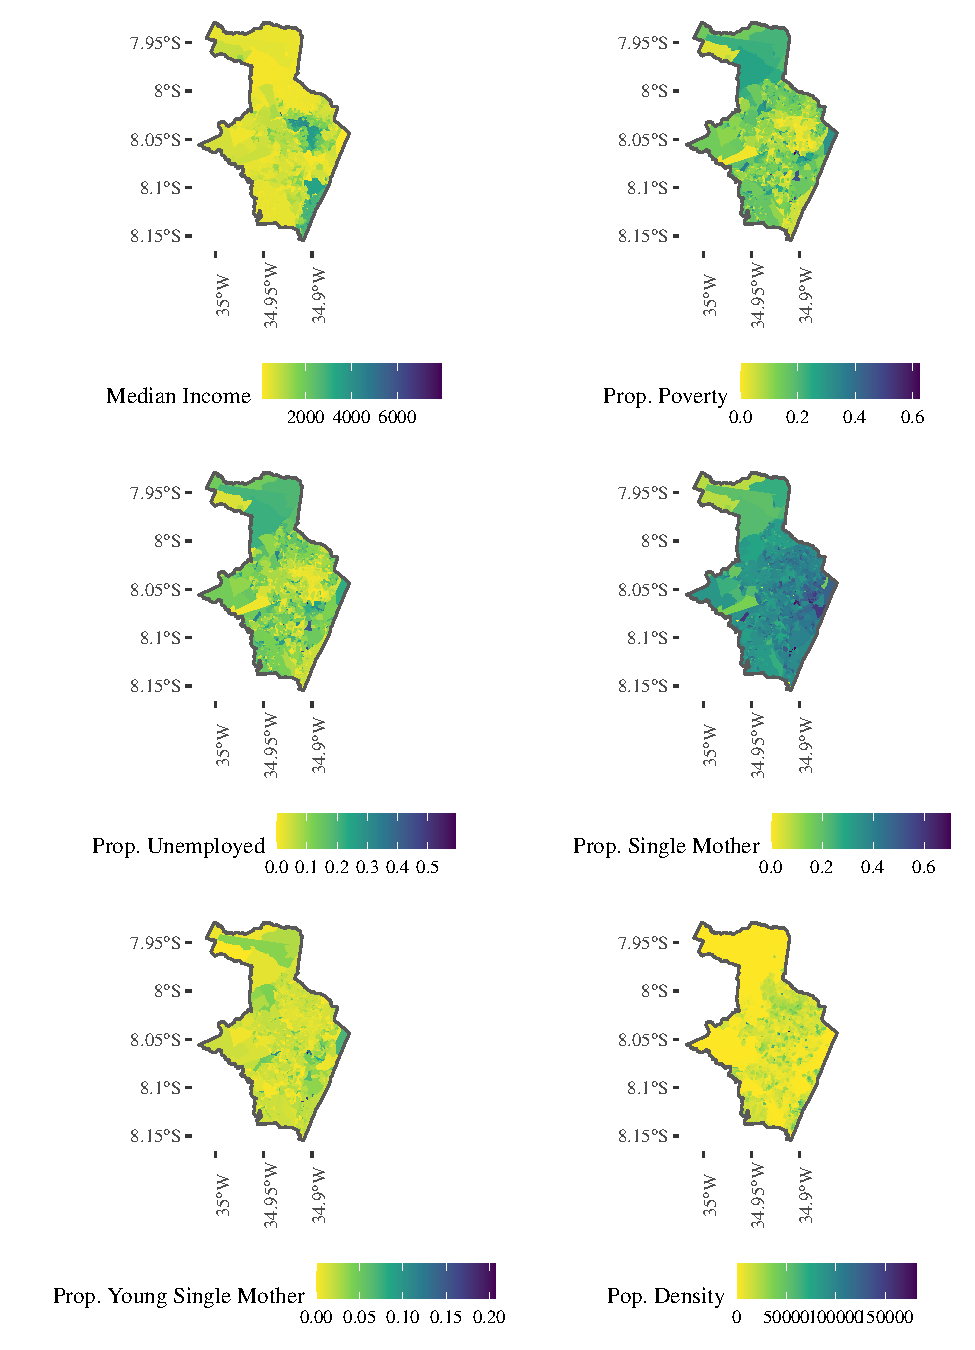
\includegraphics{Moral_Communities_and_Crime_files/figure-latex/fig-plot-sed-variables-1} \hfill{}

\caption{\label{fig:plot-sed-variables}Spatial distribution of socio-economic and demographic variables in Recife}\label{fig:fig-plot-sed-variables}
\end{figure}

For the analysis, we use Principal Component Analysis, a data reduction
technique, to obtain an indicator of Socio-Economic Deprivation,
essentially the first principal component in the output. The loadings of
this factor (Table \ref{tab:sed-descriptive-statistics}) indicate that
high Socio-Economic Deprivation is a combination of (in terms of
importance): high levels of poverty, high levels of unemployment, and
low median income, followed by high levels of family disruption, in
particular proportion of families led by young single mothers. This
factor accounts for almost 45\% of the variance.

Figure \ref{fig:plot-sed-as-quintiles} displays the geography of
Socio-Economic Deprivation in Recife, after classifying \emph{setores}
by quintiles, whereby the ``High'' class corresponds to \emph{setores}
in the top 20\% of the Socio-Economic Deprivation indicator, and the
``Low'' class corresponds to \emph{setores} in the bottom 20\% of the
Socio-Economic Deprivation indicator. The figure shows a veritable
mosaic of affluence and deprivation, with high deprivation areas
directly in contact, and in some cases almost completely surrounded, by
low deprivation areas. This geographical pattern of inequality, on the
other hand, seems to be characteristic of Brazilian metropolitan
regions, where enclaves of wealth and \emph{favelas} (i.e., urban slums)
can be found in close proximity (see for example Feitosa et al. 2007).

\begin{figure}
\centering
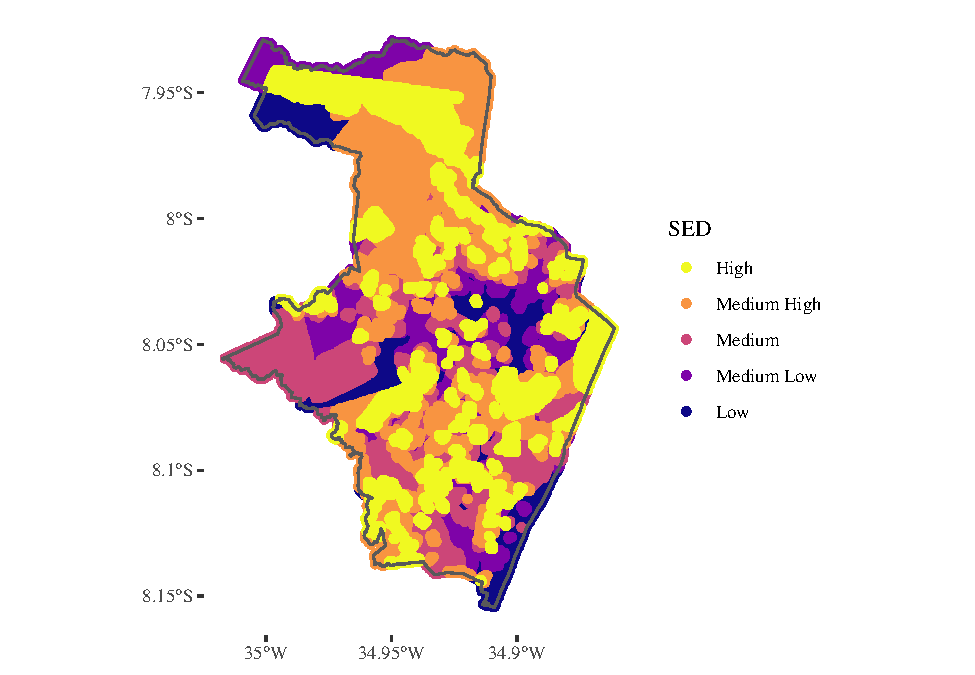
\includegraphics{Moral_Communities_and_Crime_files/figure-latex/plot-sed-as-quintiles-1.pdf}
\caption{\label{fig:plot-sed-as-quintiles}Socio-Economic Deprivation in
Recife classified by quintiles}
\end{figure}

\hypertarget{conditional-quadrat-analysis}{%
\subsection{Conditional Quadrat
Analysis}\label{conditional-quadrat-analysis}}

Once the indicator of Socio-Economic Deprivation has been obtained, as
outlined above, it can be used for conditional quadrat analysis. As
previously described, the quadrats are irregular areas that are defined
based on a covariate, in this case the quintiles of the Socio-Economic
Deprivation indicator. Each color in Figure
\ref{fig:plot-sed-as-quintiles} is a ``container'' for counting events.
In essence, this entails counting the number of events at each level of
the covariate, and then calculating an estimator of the intensity. The
global intensity of each type of event (i.e., places of worship and
businesses), as well as quadrant counts and intensity at each level of
SED can be consulted in Table \ref{tab:quadrat-count-results}.

\begin{table}

\caption{\label{tab:table-counts-intensity-summary}\label{tab:quadrat-count-results}Conditional quadrat counts results}
\centering
\begin{tabular}[t]{lcccl}
\toprule
Event & Global Intensity & SED Quintile & Quadrat Count & Intensity\\
\midrule
 &  & Low & 201 & 0\\

 &  & Middle Low & 295 & 0\\

 &  & Middle & 364 & 0\\

 &  & Middle High & 479 & 0\\

\multirow{-5}{*}{\raggedright\arraybackslash Violent Crime} &  & High & 318 & 0\\

 &  & Low & 32 & 0\\

 &  & Middle Low & 26 & 0\\

 &  & Middle & 33 & 0\\

 &  & Middle High & 29 & 0\\

\multirow{-5}{*}{\raggedright\arraybackslash Catholic} &  & High & 11 & 0\\

 &  & Low & 209 & 0\\

 &  & Middle Low & 304 & 0\\

 &  & Middle & 334 & 0\\

 &  & Middle High & 345 & 0\\

\multirow{-5}{*}{\raggedright\arraybackslash Evangelical} &  & High & 185 & 0\\

 &  & Low & 37 & 0\\

 &  & Middle Low & 50 & 0\\

 &  & Middle & 40 & 0\\

 &  & Middle High & 40 & 0\\

\multirow{-5}{*}{\raggedright\arraybackslash Spiritist} &  & High & 20 & 0\\

 &  & Low & 45 & 0\\

 &  & Middle Low & 60 & 0\\

 &  & Middle & 39 & 0\\

 &  & Middle High & 37 & 0\\

\multirow{-5}{*}{\raggedright\arraybackslash Ice Cream} &  & High & 26 & 0\\

 &  & Low & 116 & 0\\

 &  & Middle Low & 122 & 0\\

 &  & Middle & 91 & 0\\

 &  & Middle High & 84 & 0\\

\multirow{-5}{*}{\raggedright\arraybackslash Pharmacies} &  & High & 25 & 0\\

 &  & Low & 27 & 0\\

 &  & Middle Low & 32 & 0\\

 &  & Middle & 38 & 0\\

 &  & Middle High & 16 & 0\\

\multirow{-5}{*}{\raggedright\arraybackslash Super Markets} & \multirow{-35}{*}{\centering\arraybackslash 0} & High & 12 & 0\\
\bottomrule
\end{tabular}
\end{table}

Figure \ref{fig:plot-crime-quadrat} shows the results of conditional
quadrat counts for Lethal and Intentional Violent Crime. The dotted line
indicates the global intensity, simply the total number of criminal
events divided by the area of the region. It can be seen that the
intensity of crime clearly increases with Socio-Economic Deprivation,
and the intensity in areas with the highest levels of Socio-Economic
Deprivation is 216.2\% higher than in places with the lowest levels of
Socio-Economic Deprivation. This is as expected, as research has
consistently found correlations between Socio-Economic Deprivation and a
variety of negative health outcomes, including homicide (Ichihara et al.
2018). A \(\chi^2\) test of independence on the quadrat counts yields a
value of \(p\leq 0.0001\) (four degrees of freedom), which comfortably
rejects the null hypothesis of homogeneity of intensity of crime by
level of Socio-Economic Deprivation.

\begin{figure}
\centering
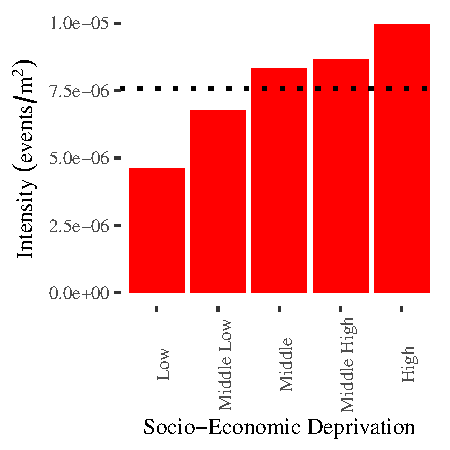
\includegraphics{Moral_Communities_and_Crime_files/figure-latex/plot-crime-quadrat-1.pdf}
\caption{\label{fig:plot-crime-quadrat}Intensity of crime by level of
Socio-Economic Deprivation; the dotted line indicates the global
intensity of crime}
\end{figure}

Next, we repeat the analysis of conditional quadrat counts, but now for
the six types of events of reference. As discussed above, this included
three types of places of worship which are of interest from the
perspective of moral communities, and three types of commercial
establishments that we posit are morally neutral. The results of
estimating the intensity of the process by means of conditional quadrat
counts are shown in Figure \ref{fig:plot-events-quadrat}.

The first thing that we note are the variations in global intensity of
places of worship, with Evangelical places of worship being the most
intense of the three. There are no clear variations in the locational
pattern of Catholic places of worship by level of Socio-Economic
Deprivation. Evangelical places of worship, on the other hand, tend to
be found more frequently in places with middle-low and middle levels of
Socio-Economic Deprivation, a pattern also discernible, albeit barely,
for Spiritist churches. Interestingly (see Table
\ref{tab:quadrat-test-statistics}) \(\chi^2\) tests of independence on
the conditional quadrat counts fail to reject the hypothesis of
homogeneity for Catholic and Spiritist churches, and it is only in the
case of Evangelical places of worship that we detect the possibility of
locational patterns that vary by level of Socio-Economic Deprivation.

Three types of commercial establishments also appear to display
inhomogeneous locational patterns (Table
\ref{tab:quadrat-test-statistics}), with the \(\chi^2\) test of
independence emphatically rejecting the null hypothesis. As seen in
Figure \ref{fig:plot-events-quadrat}, ice cream shops tend to be found
more frequently in places with middle-low Socio-Economic Deprivation,
and less frequently in places with middle-high Socio-Economic
Deprivation. Pharmacies show a clearer trend, with locational patterns
that tend to favor places with low Socio-Economic Deprivation. Finally,
supermarkets are found less frequently in places with middle-high and
high Socio-Economic Deprivation.

\begin{figure}
\centering
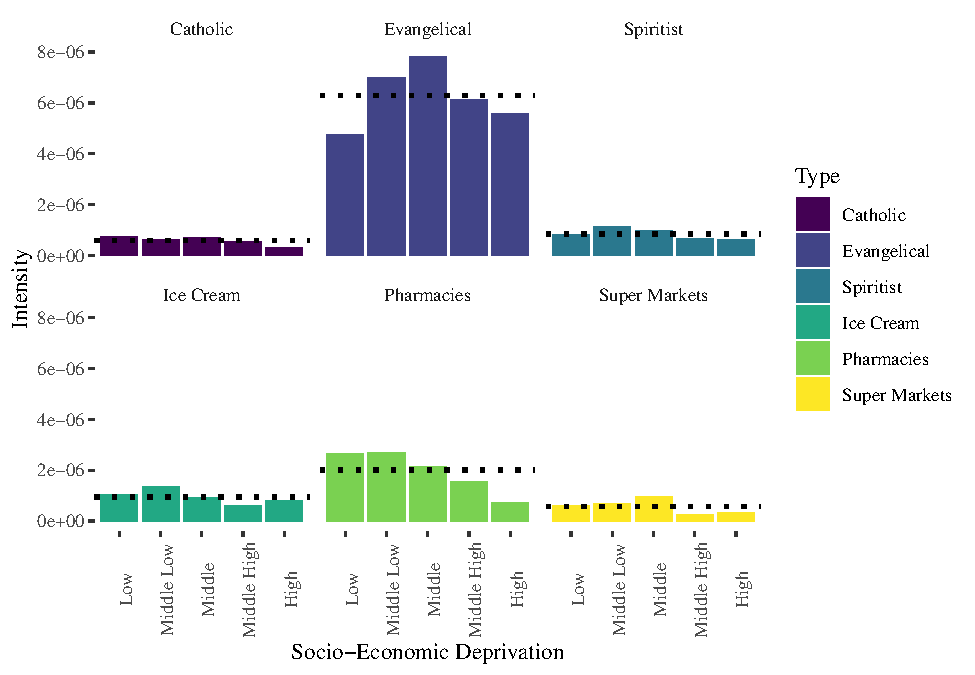
\includegraphics{Moral_Communities_and_Crime_files/figure-latex/plot-events-quadrat-1.pdf}
\caption{\label{fig:plot-events-quadrat}Intensity of places of worship
and commercial establishments by level of Socio-Economic Deprivation;
the dotted lines indicates the respective global intensities}
\end{figure}

\begin{table}

\caption{\label{tab:table-quadrat-test-statistics}\label{tab:quadrat-test-statistics}$\chi^2$ tests of independence of conditional quadrat counts}
\centering
\begin{tabular}[t]{lccc}
\toprule
Event & Statistic & Degrees of Freedom & p-value\\
\midrule
Catholic & 7.074 & 4 & 0.264\\
Evangelical & 32.976 & 4 & $<0.001$\\
Spiritist & 7.561 & 4 & 0.2181\\
Ice Cream Shop & 13.946 & 4 & 0.0149\\
Pharmacy & 53.220 & 4 & $<0.001$\\
\addlinespace
Supermarket & 18.819 & 4 & 0.0017\\
\bottomrule
\end{tabular}
\end{table}

\hypertarget{relative-distribution}{%
\subsection{Relative Distribution}\label{relative-distribution}}

The preceding analysis provides a valuable backdrop. As seen there,
there is a clear distribution of criminal events, increasing on par with
the level of Socio-Economic deprivation. Of the three different classes
of places of worship, only Evangelical churches display a locational
pattern that is commensurate, with Socio-Economic Deprivation, albeit
the pattern is distinct from criminal events, with Evangelical churches
found less frequently in both high and low Socio-Economic Deprivation
areas.

The analysis does not answer the question, yet, of possible covariations
between crime, on the one hand, and places of worship and commercial
establishments, on the other. In this subsection we implement the
relative distribution estimator of intensity of Lethal and Intentional
Violent Crime. The covariate \(Z(u)\) in this analysis is distance to
one of a place of worship or a commercial establishment: \[
\lambda_k(s)=\rho(Z_k(s))
\] with: \[
Z_k(s) = d_{sk}
\] In the expression above, \(d_{s_k}\) is distance from location \(s\)
to an event of class \(k\), and
\(k=\{\text{Catholic, Evangelical, Spiritist, Ice Cream Shop, Pharmacy, Supermarket}\}\).

The results of this analysis are shown in Figure
\ref{fig:plot-relative-distribution}. The global estimator for the
intensity of crime is shown in this figure as a dotted line. Three types
of places of worship are shown in solid lines, and three types of
commercial establishments are shown in dashed lines. Each relative
distribution function is shown with its corresponding 95\% confidence
bands.

Several interesting things emerge from inspection of this figure. First,
we notice that with the exception of Spiritist churches (which has an
intensity significantly lower than the global intensity at a distance of
zero), the intensity of crime at for other churches and commercial
establishments is close, but higher than, the global intensity of crime.
In general, the intensity tends to increase at short distances; however,
this effect is much more marked for Evangelical places of worship. The
intensity of crime in the proximity of these places of worship grows
rapidly within a short distance, reaching a peak of
\ensuremath{2.4916\times 10^{-5}} at a distance of 64.92 m. At that
distance, the intensity of crime with respect to Evangelical places of
worship is 183.78\% higher than the intensity of Catholic places of
worship; 194.54\% higher than the intensity of crime with respect to
Spiritist churches; 174.19\% higher than the intensity with respect to
ice cream shops; 151.52\% higher than the intensity with respect to
pharmacies; and 177.63\% higher than the intensity with respect to
supermarkets.

Intriguingly, after reaching its peak intensity, the intensity of crime
with respect to Evangelical places of worship declines sharply, until at
distances of approximately 200 m it is lower than for other places of
worship and commercial establishments, and at distances of approximately
270 m it is lower than the global intensity of crime. This does not
happen with other places of worship or commercial establishments: the
intensity of crime with respect to these locations remains higher than
the global intensity of crime for the interval of distances examined.
Another interesting observation is that the intensity of crime with
respect to Catholic places of worship is not substantially different
when compared to the intensity of crime with respect to any of the
commercial establishments considered.

These results, while intriguing, beg the question of whether variations
in Socio-Economic Deprivation may have a confounding effect on the
relative distributions; for instance, if as seen in the case of
conditional quadrat counts, there is some overlap in the locational
patterns of, say, Evangelical places of worship and crime with respect
to Socio-Economic Deprivation. Next section explores this question.

\begin{figure}
\centering
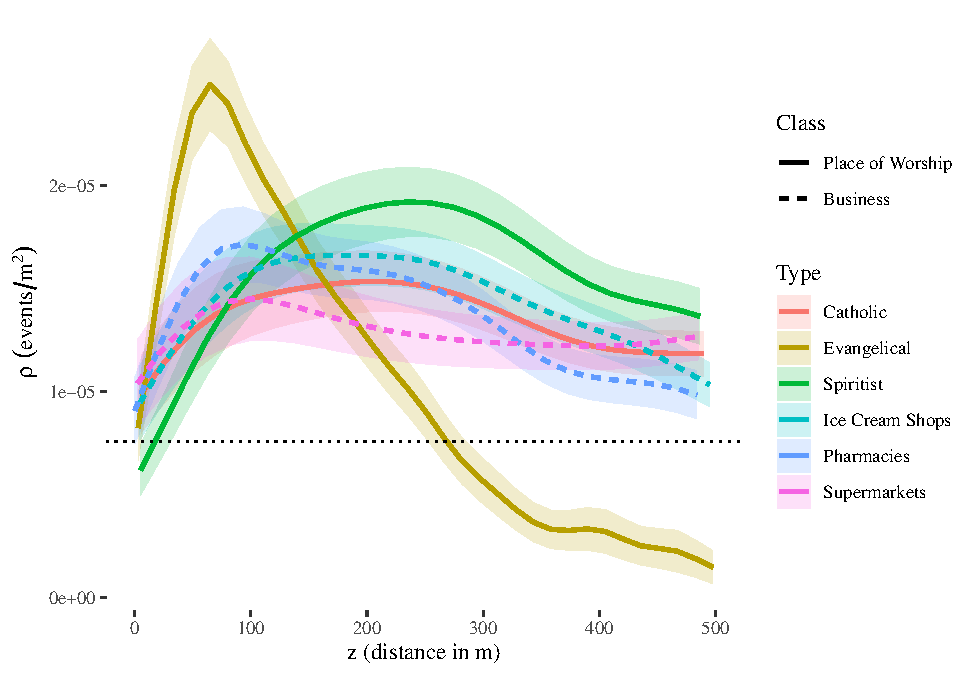
\includegraphics{Moral_Communities_and_Crime_files/figure-latex/figure-plot-relative-distribution-1.pdf}
\caption{\label{fig:plot-relative-distribution}Intensity of crime as a
function of distance to a selected place of worship or commercial
establishment; bands are 95\% confidence interval and the dotted line
indicates the global intensity of crime}
\end{figure}

\hypertarget{relative-distribution-with-a-baseline-function}{%
\subsection{Relative Distribution with a Baseline
Function}\label{relative-distribution-with-a-baseline-function}}

In this section, the preceding analysis regarding the relative
distribution of crime using distance to places of worship and commercial
establishments is repeated, after introducing a baseline function. The
interpretation of \(\rho(Z(s))\) in this case is as follows: instead of
the raw intensity at the value of \(z\), it is the intensity
\emph{relative to the intensity according to the level of Socio-Economic
Deprivation}. Therefore, \(rho(z)=1\) matches the intensity according to
Socio-Economic Deprivation; values of \(rho(z)>1\) indicate a higher
intensity than explained by Socio-Economic Deprivation; and values of
\(rho(z)<1\) correspond to lower intensities than explained by
Socio-Economic Deprivation.

The results of the analysis are shown in Figure
\ref{fig:plot-relative-distribution-with-baseline}. The general trends
shown by the relative distribution functions are similar to those seen
above, before the introduction of a baseline function. We notice that at
short distances the intensity of crime as a function of distance to the
various places of worship and commercial establishments is higher than
the baseline intensity (i.e., the intensity according to Socio-Economic
Deprivation). The only exception is intensity as a function of distance
to a Spiritist church, which at short distances is not significantly
different from the baseline intensity (see the confidence bands).

The peak intensity as a function of distance to Evangelical churches is
3.32 times the baseline intensity; for Catholic places of worship, the
highest intensity is 2.12 times the baseline intensity; and the
intensity reaches a peak of 2.67 times the baseline intensity when the
covariate is distance to Spiritist churches. Turning now to inspect the
three types of commercial establishments, we see that the highest
intensities are 2.28, 2.45, and 2.09 times the intensity according to
Socio-Economic Deprivation for ice cream shops, pharmacies, and
supermarkets, respectively.

Some differences are observed as well. Whereas the peak intensity as a
function of distance to Evangelical places of worship was 183.78\%
higher than the intensity of Catholic places of worship \emph{without a
baseline function}, once that we account for Socio-Economic Deprivation
by means of a baseline function, the peak relative intensity as a
function of distance to Evangelical churches declines to 176.48\% higher
than the intensity as a function of distance to Catholic places of
worship at the same distance. Accounting for Socio-Economic Deprivation
in this analysis of intensity has in general a moderating effect:
whereas the peak intensity of crime was was 194.54\% higher when
comparing Evangelical and Spiritist churches at the distance of the peak
intensity of Evangelical churches, this difference declines to 186.43\%
after accounting for Socio-Economic Deprivation. Similarly, this changes
from 174.19\% to 168.37\% in the case of ice cream shops, from 151.52\%
to 140.98\% in the case of pharmacies, and finally from 177.63\% to
164.31\% in the case of supermarkets.

Again, it is interesting to note that while the intensity with respect
to distance to Catholic and Spiritist places of worship, as well as ice
cream shops, pharmacies, and supermarkets remains higher than the
background intensity (given by the baseline according to Socio-Economic
Deprivation), the intensity of crime at distances of approximately 300 m
of an Evangelical church are significantly lower than the background
intensity of crime. In the following section we discuss the possible
implications of these findings.

\begin{figure}
\centering
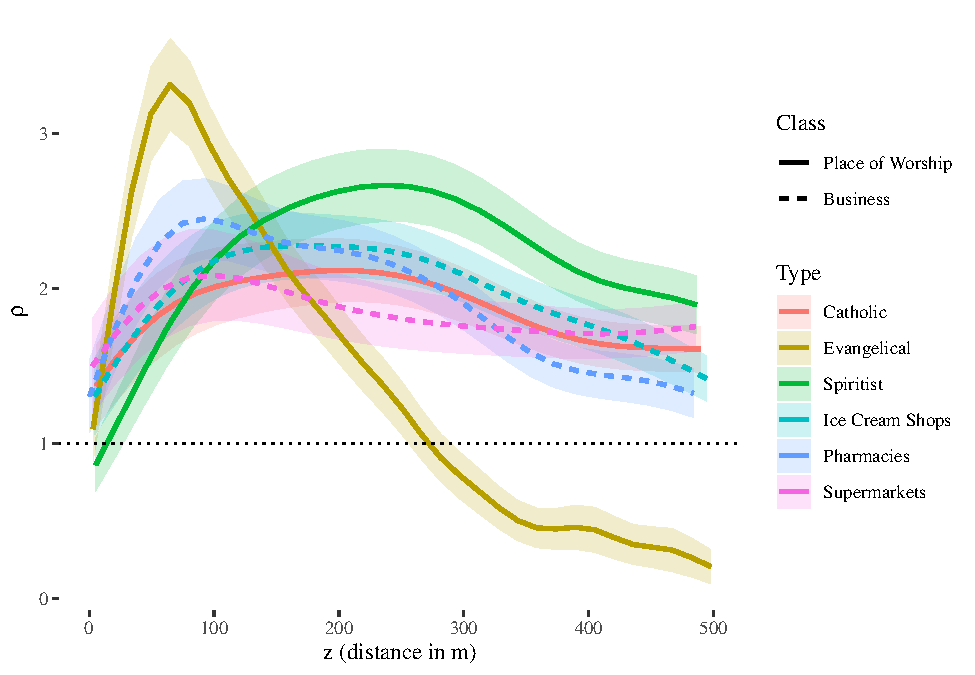
\includegraphics{Moral_Communities_and_Crime_files/figure-latex/figure-plot-relative-distribution-with-baseline-1.pdf}
\caption{\label{fig:plot-relative-distribution-with-baseline}Intensity
of crime as a function of distance to a selected place of worship or
commercial establishment after introducing Socio-Economic Deprivation as
a baseline function; bands are 95\% confidence intervals and the dotted
line indicates the baseline intensity with respect to Socio-Economic
Deprivation}
\end{figure}

\hypertarget{discussion}{%
\section{Discussion}\label{discussion}}

Theories of moral communities and social disorganization suggest that
the presence of institutions that can provide a measure of social
control can help to improve crime prevention, and this has been borne to
some extent by previous empirical research. However, as noted by Warner
and Konkel (2019), it is important to distinguish between different
religious traditions.

In this respect, it has been argued that Catholics and some Protestant
groups are more adept at generating bridging social capital with strong
intergroup relations. This can result in greater collective efficacy -
which in turn can decrease the likelihood of crime (see Hoffmann 2015,
2). Along these lines, Beyerlein and Hipp (2005), examined data for
3,157 counties in the United States in 2000, and found that counties
with greater percentages of people affiliated with mainline Protestant
and Catholic traditions tended to have lower crime rates. Similarly,
Warner and Konkel (2019) found that mainline Protestant and bridging
churches (but not Catholic churches) correlated positively with informal
social control at the neighborhood level in two cities in Kentucky. Nie
and Yang (2019), in a study of smoking, also found that share of
Catholic population in counties did not reduce the rate of smoking, thus
bringing into question the efficacy of this type of moral community in
generating social control - albeit at a fairly aggregated scale
(counties). Our findings with respect to Catholic places of worship echo
these results at a much higher level of disaggregation, as we fail to
find evidence that Catholic churches project a moral community in space
more than any of various common types of business establishments.

Conservative Protestant and Evangelic traditions, unlike mainline
Protestants and Catholics, appear to focus less on bridging and more on
bonding social capital with strong within-group relations. Associated
with this, Conservative Protestant doctrine emphasizes individual
responsibility, and therefore social ills tend to be seen as primarily
personal ills in need of religious redemption instead of secular
interventions (Nie and Yang 2019, 2--3). Under this light, a moral
community with such views of social problems may not be effective to
deter crime (Ellison, Burr, and McCall 2003); instead, conservative
Protestant doctrine may be more tolerant of violent behavior when
associated with defense of honor, family, property, or women, or
unfortunate events may be seen as representing legitimate celestial
retribution for moral turpitude. Empirical research by Beyerlein and
Hipp (2005) found that counties with greater percentages of people
affiliated with Evangelical traditions tended to have higher crime
rates. More recent research by Desmond et al.~(2010) in more than 400
block groups in Indianapolis found that neighborhoods with a greater
presence of Evangelical congregations had higher rates of both violent
and property crimes. In the specific context of Brazil, it is important
to consider the role that religion has had in interpreting and
conferring meaning to urban violence, or what Brazilian anthropologist
Patricia Birman has termed ``The Violence of the Just'' (see Birman and
Machado 2012; Birman 2019).

Our analysis suggests that the role of Evangelical churches may be more
complex than thought: on the one hand, our results indicate that Lethal
and Intentional Violent Crime tends to be more intense in the proximity
of Evangelical places of worship, up to a distance of approximately 100
m, but then declines even below the global intensity and the background
intensity at distances between 300 m and 100 m. It is at the moment
unclear what could cause this, and candidate explanations could include
the way police respond to crime incidents in different neighborhoods,
the likelihood of residents reporting crime to the police, and the level
of opportunity for crimes (Warner and Konkel 2019). Could Evangelicals
churches provide greater levels of opportunity for crime, if adherents
to this tradition are seen as meek? And is it possible that at a
different scale, unlike reports by other researchers, Evangelical
churches are more effective at keeping social control? While these
speculations cannot be answered in the context of the present study, we
suggest that these might be fruitful areas for future research.

Finally, we would like to remark on the results regarding Spiritist
churches, which in some way are the mirror image of those for
Evangelical churches. An extensive scan of the literature finds much
less information about this religious tradition, in particular in the
context of Brazil where it adapted in ways that made it very different
from its original French predecessor (see Arribas 2011b). Could it be
that Spiritism is seen by potential criminals as spiritually or
materially risky, if supernatural retribution is feared? Again, we
cannot do more than speculate about this at the moment, but this might
be another worthwhile avenue for future investigation.

\hypertarget{conclusions}{%
\section{Conclusions}\label{conclusions}}

The objective of this research was to investigate the covariation of
incidence of crime to proximity of places of worship. The hypothesis of
moral communities (closely related to social informal controls) posits a
negative correlation between the presence of churches and crime. Recent
papers have argued that it is important to study this phenomenon from a
geographical perspective, paying attention to the level of aggregation.
Accordingly, our research for the city of Recife in Brazil makes the
following contributions to the literature:

\begin{enumerate}
\def\labelenumi{\arabic{enumi}.}
\item
  By using disaggregated data for Lethal and Intentional Violent Crime
  and various types of places of worship, we were able to analyze the
  intensity of crime with respect to proximity to churches as a point
  pattern.
\item
  Following the suggestion of Warner and Konkel (2019), we also
  disaggregated our data by type of place of worship, and considered the
  three following denominations: Catholic, Evangelical, and Spiritist.
\item
  We used relative distribution functions, a multi-scale technique, that
  allowed us to estimate the intensity of crime at different distances
  from various types of places of worship.
\item
  We also used a set of putatively morally neutral commercial
  establishments to serve as controls in our analysis.
\end{enumerate}

Our key findings can be summarized as follows:

\begin{enumerate}
\def\labelenumi{\arabic{enumi}.}
\item
  Catholic places of worship do not seem to geographically project more
  or less of a moral community effect than, say, ice cream shops,
  pharmacies, or supermarkets: the intensity of crime as a function of
  distance to Catholic churches is not significantly different that what
  we observe when we consider distance to any of these types of
  commercial establishments, at any distance.
\item
  The intensity of crime with respect to distance to Evangelical
  churches is more complex than previously known: whereas the intensity
  of crime is higher at relatively short distance from Evangelical
  places of worship, at longer distances it tends to decline even below
  the global intensity of crime and the background level of crime
  according to Socio-Economic Deprivation.
\item
  Spiritist churches are associated with lower intensity of crime at
  very short distance; however, at longer distances (approximately
  between 200 m and 500 m), the intensity of crime is in fact higher
  than the intensity of crime at comparable distances from Catholic and
  Evangelical places of worship, or any of the three kinds of commercial
  establishments.
\end{enumerate}

These results are interesting in and of themselves as they help to
clarify the potential of various types of moral communities to act as
restraints on crime or, on the contrary, as criminogenic factors. They
also suggest several recommendations.

\begin{enumerate}
\def\labelenumi{\arabic{enumi}.}
\item
  The analysis presented in this paper is to a large extent exploratory.
  For example, to introduce a baseline function in the analysis of
  relative distribution, we used a data reduction technique to obtain an
  indicator of Socio-Economic Deprivation. This indicator was useful to
  determine a general spatial pattern of crime conditional on this
  variable, and to account for a baseline (or background) intensity of
  crime. However, it would be interesting to investigate the effect of
  the individual socio-economic and demographic variables on the
  intensity of crime, as opposed to the aggregated effect of
  Socio-Economic Deprivation. This implies the use of multivariate
  analytical techniques.
\item
  It would be interesting to explore the effect of aggregation on the
  results. On the one hand, this would be informative with respect to
  the well-known issues with aggregation bias in spatial analysis
  (related to the Modifiable Areal Unit Problem in geography; see
  Fotheringham and Wong 1991; Openshaw and Taylor 1979; and Tagashira
  and Okabe 2002). On the other hand, as the results of the research
  presented here, it is possible that analysis at different levels of
  aggregation may tend to capture different spatial and social processes
  of interest.
\item
  And finally, in relation to the latter point, more in-depth research,
  perhaps observational, ethnographic, or participatory studies, could
  help to develop a more refined understanding of the kinds of processes
  that operate at different scales and how they can influence moral
  behavior and crime. For example, an important question is whether the
  higher intensity of crime in the neighborhood of Evangelical churches
  is related to ``The Violence of the Just'' (see Birman and Machado
  2012; Birman 2019), or contrariwise, crime committed \emph{against}
  Evangelical Christians as a result of religious intolerance (see Souza
  2019; Fonseca 2018).
\end{enumerate}

In summary, the research presented on this paper provides information
about the potential of different types of moral communities to reduce
crime, and should be of interest to policy makers as they assess whether
formal or informal forms of social control can be effective to deter
criminal behavior, in order to achieve development goals.

\hypertarget{acknowledgments}{%
\section{Acknowledgments}\label{acknowledgments}}

The following \texttt{R} packages were used in the course of this
investigation and the authors wish to acknowledge their developers:
\texttt{faterize} (Ross 2018), \texttt{ggthemes} (Arnold 2018),
\texttt{kableExtra} (Zhu 2018), \texttt{knitr} (Xie 2015, 2018),
\texttt{maptools} (Bivand and Lewin-Koh 2019), \texttt{spatstat}
(Baddeley and Turner 2005), \texttt{raster} (Hijmans 2018),
\texttt{rticles} (Allaire et al. 2018), \texttt{sf} (Pebesma 2018), and
\texttt{tidyverse} (Wickham 2017).

\hypertarget{references}{%
\section*{References}\label{references}}
\addcontentsline{toc}{section}{References}

\hypertarget{refs}{}
\leavevmode\hypertarget{ref-Abdullah2018amenities}{}%
Abdullah, Snhs, F. A. Bohani, Z. A. Nazri, Y. Jeffry, M. A. Abdullah, M.
N. Junoh, and Z. A. Kasim. 2018. ``Amenities Surrounding Commercial
Serial Crime Prediction at Greater Valley and Kuala Lumpur Using K-Means
Clustering.'' Journal Article. \emph{Jurnal Teknologi} 80 (4): 43--53.
\url{\%3CGo\%20to\%20ISI\%3E://WOS:000437011000005}.

\leavevmode\hypertarget{ref-Allaire2018rticles}{}%
Allaire, JJ, Yihui Xie, R Foundation, Hadley Wickham, Journal of
Statistical Software, Ramnath Vaidyanathan, Association for Computing
Machinery, et al. 2018. \emph{Rticles: Article Formats for R Markdown}.
\url{https://CRAN.R-project.org/package=rticles}.

\leavevmode\hypertarget{ref-Appleyard1980livable}{}%
Appleyard, D. 1980. ``Livable Streets - Protected Neighborhoods.''
Journal Article. \emph{Annals of the American Academy of Political and
Social Science} 451 (SEP): 106--17.
\url{\%3CGo\%20to\%20ISI\%3E://A1980KK14700011}.

\leavevmode\hypertarget{ref-Arnold2018}{}%
Arnold, Jeffrey B. 2018. \emph{Ggthemes: Extra Themes, Scales and Geoms
for 'Ggplot2'}. \url{https://CRAN.R-project.org/package=ggthemes}.

\leavevmode\hypertarget{ref-Arribas2011doutrina}{}%
Arribas, Celia da Graca. 2011a. ``A Doutrina Espirita Na Formacao Da
Diversidade Religiosa Brasileira.'' \emph{Anais Do XXVI Simpósio
Nacional de História - ANPUH, Sao Paulo}.

\leavevmode\hypertarget{ref-Arribas2011espiritismo}{}%
---------. 2011b. ``Espiritismo: Entre Crime E Religiao.''
\emph{Mneme-Revista de Humanidades} 12 (29).

\leavevmode\hypertarget{ref-Baddeley2015spatial}{}%
Baddeley, Adrian, Ege Rubak, and Rolf Turner. 2015. \emph{Spatial Point
Patterns: Methodology and Applications with R}. Book. Chapman; Hall/CRC.

\leavevmode\hypertarget{ref-Baddeley2005spatstat}{}%
Baddeley, Adrian, and Rolf Turner. 2005. ``spatstat: An R Package for
Analyzing Spatial Point Patterns.'' \emph{Journal of Statistical
Software} 12 (6): 1--42. \url{http://www.jstatsoft.org/v12/i06/}.

\leavevmode\hypertarget{ref-Bailey1995interactive}{}%
Bailey, T. C., and A. C. Gatrell. 1995. \emph{Interactive Spatial Data
Analysis}. Book. Essex: Addison Wesley Longman.

\leavevmode\hypertarget{ref-Becker2017analise}{}%
Becker, Kalinca Léia, and Ana Lúcia Kassouf. 2017. ``Uma análise Do
Efeito Dos Gastos Públicos Em Educação Sobre a Criminalidade No
Brasil.'' \emph{Economia E Sociedade} 26 (1): 215--42.

\leavevmode\hypertarget{ref-Beyerlein2005social}{}%
Beyerlein, Kraig, and John R Hipp. 2005. ``Social Capital, Too Much of a
Good Thing? American Religious Traditions and Community Crime.'' Journal
Article. \emph{Social Forces} 84 (2): 995--1013.

\leavevmode\hypertarget{ref-Birman2012violencia}{}%
Birman, Patricia, and Carly Machado. 2012. ``A Violencia Dos Justos:
Evangelicos, Midia E Periferias Da Metropole.'' \emph{Revista Brasileira
de Ciências Sociais} 27 (80): 55--69.

\leavevmode\hypertarget{ref-Birman2019narrativas}{}%
Birman, Patrocia. 2019. ``NARRATIVAS Seculares E Religiosas Sobre a
Violencia: AS Fronteiras Do Humano No Governo Dos Pobres.''
\emph{Sociologia \& Antropologia} 9 (1).

\leavevmode\hypertarget{ref-Bivand2019maptools}{}%
Bivand, Roger, and Nicholas Lewin-Koh. 2019. \emph{Maptools: Tools for
Handling Spatial Objects}.
\url{https://CRAN.R-project.org/package=maptools}.

\leavevmode\hypertarget{ref-Brower2007spatial}{}%
Brower, A. M., and L. Carroll. 2007. ``Spatial and Temporal Aspects of
Alcohol-Related Crime in a College Town.'' Journal Article.
\emph{Journal of American College Health} 55 (5): 267--75.
\url{https://doi.org/10.3200/jach.55.5.267-276}.

\leavevmode\hypertarget{ref-Chesnut2017devoted}{}%
Chesnut, R Andrew. 2017. \emph{Devoted to Death: Santa Muerte, the
Skeleton Saint}. Oxford University Press.

\leavevmode\hypertarget{ref-Craglia2000comparative}{}%
Craglia, M., R. Haining, and P. Wiles. 2000. ``A Comparative Evaluation
of Approaches to Urban Crime Pattern Analysis.'' Journal Article.
\emph{Urban Studies} 37 (4): 711--29. \url{ISI:000086520800005}.

\leavevmode\hypertarget{ref-Davignon2015christian}{}%
Davignon, P., and R. A. Thomson. 2015. ``Christian Colleges and
Universities as Moral Communities: The Effects of Institutional
Characteristics on Student Religiosity.'' Journal Article. \emph{Review
of Religious Research} 57 (4): 531--54.
\url{https://doi.org/10.1007/s13644-015-0214-5}.

\leavevmode\hypertarget{ref-Deryol2016crime}{}%
Deryol, R., P. Wilcox, M. Logan, and J. Wooldredge. 2016. ``Crime Places
in Context: An Illustration of the Multilevel Nature of Hot Spot
Development.'' Journal Article. \emph{Journal of Quantitative
Criminology} 32 (2): 305--25.
\url{https://doi.org/10.1007/s10940-015-9278-1}.

\leavevmode\hypertarget{ref-Desmond2010congregations}{}%
Desmond, S. A., G. Kikuchi, and K. H. Morgan. 2010. ``Congregations and
Crime: Is the Spatial Distribution of Congregations Associated with
Neighborhood Crime Rates?'' Journal Article. \emph{Journal for the
Scientific Study of Religion} 49 (1): 37--55.
\url{https://doi.org/10.1111/j.1468-5906.2009.01491.x}.

\leavevmode\hypertarget{ref-Donovan1986different}{}%
Donovan, Peter. 1986. ``Do Different Religions Share Moral Common
Ground?'' Journal Article. \emph{Religious Studies} 22 (3/4): 367--75.
\url{http://www.jstor.org.libaccess.lib.mcmaster.ca/stable/20006295}.

\leavevmode\hypertarget{ref-Doran2011putting}{}%
Doran, Bruce J, and Melissa B Burgess. 2011. \emph{Putting Fear of Crime
on the Map: Investigating Perceptions of Crime Using Geographic
Information Systems}. Springer Science \& Business Media.

\leavevmode\hypertarget{ref-Durrant2017religion}{}%
Durrant, Russil, and Zoe Poppelwell. 2017. ``Why Religion Matters.'' In
\emph{Religion, Crime and Punishment}, 1--17. Springer.

\leavevmode\hypertarget{ref-Eitle2011religion}{}%
Eitle, D. 2011. ``Religion and Gambling Among Young Adults in the United
States: Moral Communities and the Deterrence Hypothesis.'' Journal
Article. \emph{Journal for the Scientific Study of Religion} 50 (1):
61--81. \url{https://doi.org/10.1111/j.1468-5906.2010.01552.x}.

\leavevmode\hypertarget{ref-Ellison2003enduring}{}%
Ellison, Christopher G, Jeffrey A Burr, and Patricia L McCall. 2003.
``The Enduring Puzzle of Southern Homicide: Is Regional Religious
Culture the Missing Piece?'' \emph{Homicide Studies} 7 (4): 326--52.

\leavevmode\hypertarget{ref-Feitosa2007global}{}%
Feitosa, F. F., G. Camara, A. M. V. Monteiro, T. Koschitzki, and M. P.
S. Silva. 2007. ``Global and Local Spatial Indices of Urban
Segregation.'' Journal Article. \emph{International Journal of
Geographical Information Science} 21 (3): 299--323.
\url{ISI:000244944300004\%0AC:/Papers/International\%20Journal\%20of\%20Geographical\%20Information\%20Science/IJGIS\%20(2007)\%2021\%20(3)\%20299-323.pdf}.

\leavevmode\hypertarget{ref-Fonseca2018primeiras}{}%
Fonseca, Alexandre Brasil. 2018. ``Primeiras Análises Dos Dados Do
Relatório Sobre Intolerância E Violência Religiosa No Brasil
(2011-2015).'' Journal Article. \emph{Estado Laico, Intolerância E
Diversidade Religiosa No Brasil. Brasília, Ministério Dos Direitos
Humanos}, 22--47.

\leavevmode\hypertarget{ref-Foster2010neighbourhood}{}%
Foster, S., B. Giles-Corti, and M. Knuiman. 2010. ``Neighbourhood Design
and Fear of Crime: A Social-Ecological Examination of the Correlates of
Residents' Fear in New Suburban Housing Developments.'' Journal Article.
\emph{Health \& Place} 16 (6): 1156--65.
\url{https://doi.org/10.1016/j.healthplace.2010.07.007}.

\leavevmode\hypertarget{ref-Fotheringham1991modifiable}{}%
Fotheringham, A. S., and D. W. S. Wong. 1991. ``The Modifiable Areal
Unit Problem in Multivariate Statistical-Analysis.'' Journal Article.
\emph{Environment and Planning A} 23 (7): 1025--44.
\url{ISI:A1991GA61200008}.

\leavevmode\hypertarget{ref-Furr2010metric}{}%
Furr-Holden, C. D. M., K. D. M. Campbell, A. J. Milam, M. J. Smart, N.
A. Ialongo, and P. J. Leaf. 2010. ``Metric Properties of the
Neighborhood Inventory for Environmental Typology (Nifety): An
Environmental Assessment Tool for Measuring Indicators of Violence,
Alcohol, Tobacco, and Other Drug Exposures.'' Journal Article.
\emph{Evaluation Review} 34 (3): 159--84.
\url{https://doi.org/10.1177/0193841x10368493}.

\leavevmode\hypertarget{ref-Garmany2014space}{}%
Garmany, J. 2014. ``Space for the State? Police, Violence, and Urban
Poverty in Brazil.'' Journal Article. \emph{Annals of the Association of
American Geographers} 104 (6): 1239--55.
\url{https://doi.org/10.1080/00045608.2014.944456}.

\leavevmode\hypertarget{ref-Gilbertson2012engineering}{}%
Gilbertson, Alan, and Alan Hayes. 2012. ``Engineering to Reduce Crime
and Disorder in Public Places.'' In \emph{Proceedings of the Institution
of Civil Engineers-Municipal Engineer}, 165:175--83. 3. Thomas Telford
Ltd.

\leavevmode\hypertarget{ref-Grannis2009from}{}%
Grannis, R. 2009. \emph{From the Ground up: Translating Geography into
Community Through Neighbor Networks}. Book. Princeton: Princeton
University Press.

\leavevmode\hypertarget{ref-Groff2015informal}{}%
Groff, E. R. 2015. ``Informal Social Control and Crime Events.'' Journal
Article. \emph{Journal of Contemporary Criminal Justice} 31 (1):
90--106. \url{https://doi.org/10.1177/1043986214552619}.

\leavevmode\hypertarget{ref-He2017built}{}%
He, Li, Antonio Páez, and Desheng Liu. 2017. ``Built Environment and
Violent Crime: An Environmental Audit Approach Using Google Street
View.'' Journal Article. \emph{Computers, Environment and Urban Systems}
66: 83--95.
\url{https://doi.org/http://dx.doi.org/10.1016/j.compenvurbsys.2017.08.001}.

\leavevmode\hypertarget{ref-He2015temporal}{}%
He, L., A. Paez, D. S. Liu, and S. G. Jiang. 2015. ``Temporal Stability
of Model Parameters in Crime Rate Analysis: An Empirical Examination.''
Journal Article. \emph{Applied Geography} 58: 141--52.
\url{https://doi.org/10.1016/j.apgeog.2015.02.002}.

\leavevmode\hypertarget{ref-Hijmans2018raster}{}%
Hijmans, Robert J. 2018. \emph{Raster: Geographic Data Analysis and
Modeling}. \url{https://CRAN.R-project.org/package=raster}.

\leavevmode\hypertarget{ref-Hipp2007block}{}%
Hipp, J. R. 2007. ``Block, Tract, and Levels of Aggregation:
Neighborhood Structure and Crime and Disorder as a Case in Point.''
Journal Article. \emph{American Sociological Review} 72 (5): 659--80.
\url{https://doi.org/10.1177/000312240707200501}.

\leavevmode\hypertarget{ref-Hirschi1969hellfire}{}%
Hirschi, Travis, and Rodney Stark. 1969. ``Hellfire and Delinquency.''
\emph{Social Problems} 17 (2): 202--13.

\leavevmode\hypertarget{ref-Hoffmann2015religion}{}%
Hoffmann, John P. 2015. ``Religion and Crime.'' \emph{The Encyclopedia
of Crime and Punishment}, 1--5.

\leavevmode\hypertarget{ref-Ichihara2018area}{}%
Ichihara, M. Y. T., D. Ramos, P. Reboucas, F. J. Oliveira, A. J. F.
Ferreira, C. Teixeira, M. Allik, et al. 2018. ``Area Deprivation
Measures Used in Brazil: A Scoping Review.'' Journal Article.
\emph{Revista de Saude Publica} 52 (83): 1--14.
\url{https://doi.org/10.11606/s1518-8787.2018052000933}.

\leavevmode\hypertarget{ref-Jacobs1961death}{}%
Jacobs, Jane. 1961. \emph{The Death and Life of Great American Cities}.
Book. New York: Vintage.

\leavevmode\hypertarget{ref-Jacobs1968community}{}%
---------. 1968. ``Community on the City Streets.'' Book Section. In
\emph{The Search for Community in Modern America}, edited by D.
Baltzell, 74--93. New York: Harper \& Row.

\leavevmode\hypertarget{ref-Johnson2011more}{}%
Johnson, Byron. 2011. \emph{More God, Less Crime: Why Faith Matters and
How It Could Matter More}. Templeton Foundation Press.

\leavevmode\hypertarget{ref-Kiani2015analysis}{}%
Kiani, Rasoul, Siamak Mahdavi, and Amin Keshavarzi. 2015. ``Analysis and
Prediction of Crimes by Clustering and Classification.''
\emph{International Journal of Advanced Research in Artificial
Intelligence} 4 (8): 11--17.

\leavevmode\hypertarget{ref-Lee2004love}{}%
Lee, M. R., and J. P. Bartkowski. 2004. ``Love Thy Neighbor? Moral
Communities, Civic Engagement, and Juvenile Homicide in Rural Areas.''
Journal Article. \emph{Social Forces} 82 (3): 1001--35.
\url{https://doi.org/10.1353/sof.2004.0044}.

\leavevmode\hypertarget{ref-Levine1986crime}{}%
Levine, Ned, Martin Wachs, and Elham Shirazi. 1986. ``Crime at Bus
Stops: A Study of Environmental Factors.'' \emph{Journal of
Architectural and Planning Research}, 339--61.

\leavevmode\hypertarget{ref-Lipton2008spatial}{}%
Lipton, R., A. Banerjee, D. Levy, N. Manzanilla, and M. Cochrane. 2008.
``The Spatial Distribution of Underage Tobacco Sales in Los Angeles.''
Journal Article. \emph{Substance Use \& Misuse} 43 (11): 1597--1617.
\url{https://doi.org/10.1080/10826080802241110}.

\leavevmode\hypertarget{ref-Loukaitou2001measuring}{}%
Loukaitou-Sideris, A., R. Liggett, H. Iseki, and W. Thurlow. 2001.
``Measuring the Effects of Built Environment on Bus Stop Crime.''
Journal Article. \emph{Environment and Planning B-Planning \& Design} 28
(2): 255--80. \url{https://doi.org/10.1068/b2642r}.

\leavevmode\hypertarget{ref-Malleson2015spatio}{}%
Malleson, Nick, and Martin A Andresen. 2015. ``Spatio-Temporal Crime
Hotspots and the Ambient Population.'' \emph{Crime Science} 4 (1): 10.

\leavevmode\hypertarget{ref-Malleson2019identifying}{}%
Malleson, N., W. Steenbeek, and M. A. Andresen. 2019. ``Identifying the
Appropriate Spatial Resolution for the Analysis of Crime Patterns.''
Journal Article. \emph{Plos One} 14 (6).
\url{https://doi.org/10.1371/journal.pone.0218324}.

\leavevmode\hypertarget{ref-Menezes2013spatial}{}%
Menezes, T., R. Silveira-Neto, C. Monteiro, and J. L. Ratton. 2013.
``Spatial Correlation Between Homicide Rates and Inequality: Evidence
from Urban Neighborhoods.'' Journal Article. \emph{Economics Letters}
120 (1): 97--99. \url{https://doi.org/10.1016/j.econlet.2013.03.040}.

\leavevmode\hypertarget{ref-Mora2008marketing}{}%
Mora, G. Cristina. 2008. ``Marketing the `Health and Wealth Gospel'
Across National Borders; Evidence from Brazil and the United States.''
\emph{Poetics} 36 (5): 404--20.
\url{https://doi.org/https://doi.org/10.1016/j.poetic.2008.06.008}.

\leavevmode\hypertarget{ref-Murray2013crime}{}%
Murray, J., D. R. D. Cerqueira, and T. Kahn. 2013. ``Crime and Violence
in Brazil: Systematic Review of Time Trends, Prevalence Rates and Risk
Factors.'' Journal Article. \emph{Aggression and Violent Behavior} 18
(5): 471--83. \url{https://doi.org/10.1016/j.avb.2013.07.003}.

\leavevmode\hypertarget{ref-Nakaya2010visualizing}{}%
Nakaya, T., and K. J. Yano. 2010. ``Visualising Crime Clusters in a
Space-Time Cube: An Exploratory Data-Analysis Approach Using Space-Time
Kernel Density Estimation and Scan Statistics.'' Journal Article.
\emph{Transactions in Gis} 14 (3): 223--39.
\url{https://doi.org/10.1111/j.1467-9671.2010.01194.x}.

\leavevmode\hypertarget{ref-Nie2019smoking}{}%
Nie, F. H., and X. Z. Y. Yang. 2019. ``Smoking in the Temple of the Holy
Spirit? Geographic Location Matters.'' Journal Article. \emph{Health \&
Place} 58. \url{https://doi.org/10.1016/j.healthplace.2019.05.017}.

\leavevmode\hypertarget{ref-Openshaw1979million}{}%
Openshaw, S., and P. J. Taylor. 1979. ``A Million or so Correlation
Coefficients: Three Experiments on the Modifiable Areal Unit Problem.''
Book Section. In \emph{Statistical Applications in the Spatial
Sciences}, edited by N. Wrigley, 127--44. London: Pion.

\leavevmode\hypertarget{ref-Paez2013mapping}{}%
Paez, A. 2013. ``Mapping Travelers' Attitudes: Does Space Matter?''
Journal Article. \emph{Journal of Transport Geography} 26: 117--25.
\url{https://doi.org/10.1016/j.jtrangeo.2012.09.002}.

\leavevmode\hypertarget{ref-Pebesma2018simple}{}%
Pebesma, Edzer. 2018. ``Simple Features for R: Standardized Support for
Spatial Vector Data.'' \emph{The R Journal} 10 (1): 439--46.
\url{https://doi.org/10.32614/RJ-2018-009}.

\leavevmode\hypertarget{ref-Quick2017influence}{}%
Quick, M., J. Law, and H. Luan. 2017. ``The Influence of on-Premise and
Off-Premise Alcohol Outlets on Reported Violent Crime in the Region of
Waterloo, Ontario: Applying Bayesian Spatial Modeling to Inform Land Use
Planning and Policy.'' Journal Article. \emph{Applied Spatial Analysis
and Policy} 10 (3): 435--54.
\url{https://doi.org/10.1007/s12061-016-9191-5}.

\leavevmode\hypertarget{ref-Regnerus2003moral}{}%
Regnerus, M. D. 2003. ``Moral Communities and Adolescent Delinquency:
Religious Contexts and Community Social Control.'' Journal Article.
\emph{Sociological Quarterly} 44 (4): 523--54.
\url{\%3CGo\%20to\%20ISI\%3E://WOS:000188319800001}.

\leavevmode\hypertarget{ref-Reiss1951delinquency}{}%
Reiss, Albert J. 1951. ``Delinquency as the Failure of Personal and
Social Controls.'' Journal Article. \emph{American Sociological Review}
16 (2): 196--207. \url{https://doi.org/10.2307/2087693}.

\leavevmode\hypertarget{ref-Ripley1976second}{}%
Ripley, B. D. 1976. ``The Second-Order Analysis of Stationary Point
Processes.'' Journal Article. \emph{Journal of Applied Probability} 13
(2): 255--66. \url{ISI:A1976CA37400007}.

\leavevmode\hypertarget{ref-Rogerson2001spatial}{}%
Rogerson, Peter, and Y Sun. 2001. ``Spatial Monitoring of Geographic
Patterns: An Application to Crime Analysis.'' \emph{Computers,
Environment and Urban Systems} 25 (6): 539--56.

\leavevmode\hypertarget{ref-Rohrbaugh1975religiosity}{}%
Rohrbaugh, John, and Richard Jessor. 1975. ``Religiosity in Youth: A
Personal Control Against Deviant Behavior.'' \emph{Journal of
Personality} 43 (1): 136--55.

\leavevmode\hypertarget{ref-Ross2018fasterize}{}%
Ross, Noam. 2018. \emph{Fasterize: Fast Polygon to Raster Conversion}.
\url{https://CRAN.R-project.org/package=fasterize}.

\leavevmode\hypertarget{ref-deSouza2019pluralidade}{}%
Souza, André Ricardo de. 2019. ``Pluralidade Cristã E Algumas Questões
Do Cenário Religioso Brasileiro.'' \emph{Revista USP}, no. 120: 13--22.

\leavevmode\hypertarget{ref-Stark1996religion}{}%
Stark, R. 1996. ``Religion as Context: Hellfire and Delinquency One More
Time.'' Journal Article. \emph{Sociology of Religion} 57 (2): 163--73.
\url{https://doi.org/10.2307/3711948}.

\leavevmode\hypertarget{ref-Stroope2018moral}{}%
Stroope, S., and J. O. Baker. 2018. ``Whose Moral Community?
Religiosity, Secularity, and Self-Rated Health Across Communal Religious
Contexts.'' Journal Article. \emph{Journal of Health and Social
Behavior} 59 (2): 185--99.
\url{https://doi.org/10.1177/0022146518755698}.

\leavevmode\hypertarget{ref-Tagashira2002modifiable}{}%
Tagashira, N., and A. Okabe. 2002. ``The Modifiable Areal Unit Problem
in a Regression Model Whose Independent Variable Is a Distance from a
Predetermined Point.'' Journal Article. \emph{Geographical Analysis} 34
(1): 1--20. \url{ISI:000173383000001}.

\leavevmode\hypertarget{ref-Taylor1988human}{}%
Taylor, Ralph B. 1988. \emph{Human Territorial Functioning: An
Empirical, Evolutionary Perspective on Individual and Small Group
Territorial Cognitions, Behaviors, and Consequences}. Book. Cambridge
University Press.

\leavevmode\hypertarget{ref-Taylor1998crime}{}%
Taylor, Ralph B. 1998. ``Crime and Small-Scale Places: What We Know,
What We Can Prevent, and What Else We Need to Know.'' Book Section. In
\emph{Crime and Place: Plenary Papers of the 1997 Conference on Criminal
Justice Research and Evaluation}, edited by Ralph B. Taylor, 1--22.
Washington, D.C.: National Institute of Justice.

\leavevmode\hypertarget{ref-Topalli2013god}{}%
Topalli, V., T. Brezina, and M. Bernhardt. 2013. ``With God on My Side:
The Paradoxical Relationship Between Religious Belief and Criminality
Among Hardcore Street Offenders.'' Journal Article. \emph{Theoretical
Criminology} 17 (1): 49--69.
\url{https://doi.org/10.1177/1362480612463114}.

\leavevmode\hypertarget{ref-Traunmuller2011moral}{}%
Traunmuller, R. 2011. ``Moral Communities? Religion as a Source of
Social Trust in a Multilevel Analysis of 97 German Regions.'' Journal
Article. \emph{European Sociological Review} 27 (3): 346--63.
\url{https://doi.org/10.1093/esr/jcq011}.

\leavevmode\hypertarget{ref-Unodc2019executive}{}%
United Nations Office on Drugs and Crime. 2019a. ``Global Study on
Homicide 2019: Executive Summary.'' UNODC Vienna.

\leavevmode\hypertarget{ref-Unodc2019development}{}%
---------. 2019b. ``Global Study on Homicide 2019: Homicide, Development
and the Sustainable Development Goals.'' UNODC Vienna.

\leavevmode\hypertarget{ref-Warner2019neighborhood}{}%
Warner, B. D., and R. H. Konkel. 2019. ``Neighborhood Churches and Their
Relationship to Neighborhood Processes Important for Crime Prevention.''
Journal Article. \emph{Journal of Urban Affairs}.
\url{https://doi.org/10.1080/07352166.2019.1581030}.

\leavevmode\hypertarget{ref-Wickham2017}{}%
Wickham, Hadley. 2017. \emph{Tidyverse: Easily Install and Load the
'Tidyverse'}. \url{https://CRAN.R-project.org/package=tidyverse}.

\leavevmode\hypertarget{ref-Xie2015}{}%
Xie, Yihui. 2015. \emph{Dynamic Documents with R and Knitr}. 2nd ed.
Boca Raton, Florida: Chapman; Hall/CRC. \url{https://yihui.name/knitr/}.

\leavevmode\hypertarget{ref-Xie2018}{}%
---------. 2018. \emph{Knitr: A General-Purpose Package for Dynamic
Report Generation in R}. \url{https://yihui.name/knitr/}.

\leavevmode\hypertarget{ref-Zhu2018}{}%
Zhu, Hao. 2018. \emph{KableExtra: Construct Complex Table with 'Kable'
and Pipe Syntax}. \url{https://CRAN.R-project.org/package=kableExtra}.

\bibliographystyle{spbasic}
\bibliography{bibliography.bib}

\end{document}
